\documentclass[a4paper,11pt]{article}

\usepackage[utf8]{inputenc}
\usepackage[T1]{fontenc} 
\usepackage[brazilian]{babel}

\usepackage{caption}
\captionsetup{skip=2pt}

\usepackage{vhistory}
\renewcommand \vhAuthorColWidth{1.0\hsize}
\renewcommand \vhChangeColWidth{1.0\hsize}

\usepackage{lmodern} 
\usepackage{microtype}
\usepackage{graphicx}
\usepackage{enumitem}
\setlist{leftmargin=*}
\usepackage{listings}
\usepackage{xcolor}
\usepackage{float}

\usepackage[os=win]{menukeys}
\renewmenumacro{\keys}[+]{shadowedroundedkeys}
\usepackage{framed}
\usepackage{etoolbox}
\AtBeginEnvironment{leftbar}{\sffamily}

\usetikzlibrary{chains,arrows,shapes,positioning}
\usepackage[obeyspaces]{url}
\usepackage[colorlinks=true, linkcolor=blue, urlcolor=blue]{hyperref}

\usepackage[margin=1in]{geometry}
\usepackage{indentfirst}

\usepackage{mdframed}   % For the frame

\newcommand{\sistema}{\textsf{SIRERC}}
\newcommand{\cmake}{\textit{CMake}}
\newcommand{\build}{\textit{build}}
\newcommand{\qtcreator}{\textit{Qt Creator}}
\newcommand{\qtdesigner}{\textit{Qt Designer}}
\newcommand{\qt}{\textit{Qt}}
\newcommand{\vscode}{\textit{VSCode}}
\newcommand{\msvs}{\textit{Microsoft Visual Studio}}
\newcommand{\visualstudio}{\textit{Visual Studio}}
\newcommand{\msvc}{\textit{MSVC}}
\newcommand{\gmsh}{\textit{Gmsh}}
\newcommand{\download}{\textit{Download}}
\newcommand{\windows}{\textit{Windows}}
\newcommand{\linux}{\textit{Linux}}
\newcommand{\mac}{\textit{MacOS}}
\newcommand{\gnu}{\textit{GNU General Public License}}
\newcommand{\qtfive}{\textit{Qt 5.15.2}}
\newcommand{\mongo}{\textit{MongoDB}}
\newcommand{\github}{\textit{GitHub}}

\newcommand{\cautionbox}[1]{
	\vskip 5mm
	\begin{leftbar}
		\textbf{#1}
	\end{leftbar}
	\vskip 5mm
}

\title{Guia de instalação dos ambientes de desenvolvimento do \sistema{}}

\date{\url{https://github.com/sirercita/SIRERC\_ProjetoPetrobrasdocs/}}

\begin{document}
\maketitle

\begin{versionhistory}
  \vhEntry{0.1.0}{28/08/2023}{André F. M. Caetano}{Primeira versão.}
  \vhEntry{0.2.0}{04/09/2023}{André F. M. Caetano}{Nova seção para instalador.}
  \vhEntry{0.3.0}{25/09/2023}{André F. M. Caetano}{Nova seção \gmsh{}, atualização de versões.}
  \vhEntry{0.4.0}{27/04/2024}{Nicolas F. C. Granese}{Nova seção WSL, melhorias na seção compilação do código.}
  \vhEntry{0.5.0}{02/09/2024}{A. Celio P. Mesquita}{Atualização da instalação do ambiente de desenvolvimento}
\end{versionhistory}

\newpage
\begin{abstract}
	O \textit{front-end} de um software de simulação deve prover uma interface de usuário intuitiva e organizada que facilite a definição dos cenários a serem simulados.
	
	\sistema{} é uma interface humano-máquina (\emph{HMI - Human-Machine Interface}) para definição de cenários em dinâmica de fluidos computacional (\textit{Computational Fluid Dynamics — CFD}).
	
	Este é o guia de instalação dos ambientes de desenvolvimentos do \sistema{}.
\end{abstract}


\newpage
\tableofcontents

\newpage

\section{INSTALAÇÃO DO AMBIENTE WINDOWS}

O \sistema{} é uma aplicação \emph{desktop} baseada na versão \emph{open-source} do \emph{framework} \qt{}, escolhido pela sua portabilidade, capacidade de gerar aplicações multiplataforma para sistemas MS \windows{}, \linux{} e \mac{}. A linguagem de programação utilizada é C++.

Este manual foi atualizado por meio das instalações em duas máquina com \textit{Windows 11 Pro} com versões diferentes.

\subsection{GitHub e LaTeX}

\begin{enumerate}
	
	\item **GitHub Desktop**
	\begin{enumerate}
		\item Baixe e instale o \textit{GitHub Desktop} do endereço: \url{https://desktop.github.com/download/}
		\item Ao abrir a tela de instalação entre com o sua conta do \github{}.
		\item Clone ou atualize o projeto de interesse.
	\end{enumerate}

	\item **LaTeX** {\color{blue}apenas para quem estiver encarregado de atualizar este manual.}

		Baixe e instale um editor de \textit{LaTeX}. Pode ser este \url{https://www.texstudio.org/} ou outro da sua preferência.

\end{enumerate}


\subsection{Instalação do \emph{WSL} (opcional)}

O \textit{WSL} (\textit{Windows Subsystem for Linux}) permite que desenvolvedores executem um ambiente \textit{GNU/Linux} diretamente no \windows{}, sem a necessidade de uma máquina virtual ou \textit{dual-boot}.

Utilizar o WSL facilita o seguimento de processos e ferramentas já usados por colegas que desenvolvem em sistemas \textit{Linux}, tornando a colaboração em projetos mais integrada e eficiente.

\begin{enumerate}
	
	\item **Instalação do WSL:**
	\begin{enumerate}
		\item Abra o \textit{PowerShell} ou o \textit{Prompt de Comando} do \windows{} no modo administrador clicando com o botão direito do mouse e selecionando "Executar como administrador".
		\item Insira o comando \texttt{wsl --install} e pressione \keys{Enter}. Este comando instalará o WSL e a distribuição padrão do Linux. Após a instalação, reinicie o computador.
	\end{enumerate}
	
	\begin{figure}[H]
		\centering
		\fbox{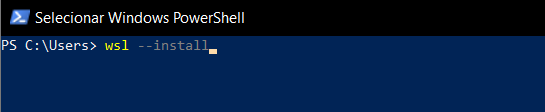
\includegraphics[width=0.75\textwidth]{images/prompt_wsl.png}}
		\caption{Comando para instalar o WSL no \windows{}}\label{fig:prompt_wsl}
	\end{figure}
	
	\item **Verificação da Instalação:**
	\begin{enumerate}
		\item Após reiniciar o computador, abra novamente o \textit{PowerShell} ou o \textit{Prompt de Comando} e insira o comando \texttt{wsl} para verificar se o WSL foi instalado corretamente.
		\item Se o WSL estiver instalado corretamente, um prompt de linha de comando do Linux será exibido. Você pode usar esse ambiente para executar comandos do Linux e interagir com o sistema de arquivos do \windows{}.
	\end{enumerate}
	
\end{enumerate}


\subsection{\textit{Download} e instalação da versão \qtfive{}}
\label{qt5}

Primeiramente, será preciso instalar o \qt{} versão 5.15.x, padrão atual para desenvolvimento do \sistema{}, bem como as versões corretas dos \textit{drivers} do C++. Assim, quando se for instalar o \qtcreator{}, as bibliotecas necessárias já estarão instaladas para permitir a configuração exata do projeto.


\subsubsection{Instalação dos requisitos de desenvolvimento}

Há ainda, algumas linguagens de programação e ferramentas que serão utilizadas direta ou indiretamente nas compilações e no desenvolvimento do \sistema{}.

\begin{itemize}
	\item Perl
	\item Python
	\item Ruby
	\item Compilador C++ com suporte ao padrão C++11 e compatível com o \qt{} 5.15.x
	\item CMake
	\item Git
\end{itemize}

\subsubsection{Instalando o ambiente \textit{ActiveState}}

\textit{ActiveState} é uma empresa de software que fornece distribuições de linguagens de programação \textit{open source}, como \textit{Python}, \textit{Perl}, \textit{Ruby} e \textit{Tcl}. Essas distribuições são pré-configuradas e testadas para garantir compatibilidade e desempenho em diferentes sistemas operacionais.

Em resumo, \textit{ActiveState} é uma solução que simplifica o processo de desenvolvimento e implantação de aplicativos usando linguagens de programação \textit{open source}.

Crie uma conta, uma organização e um projeto para cada linguagem de programação no \textit{ActiveState}. A conta poderá ser o seu e-mail e a organização o seu nome.

Ao criar um projeto aparecerá esta tela para instalação do ambiente do \textit{ActiveState}. Faça o download e a instalação.
\begin{figure}[H]
	\centering
	\fbox{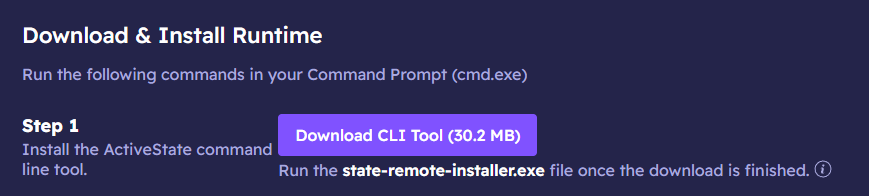
\includegraphics[width=0.95\textwidth]{images/activeState_install}}
	\caption{Instalação do ambiente \textit{ActiveState}}
	\label{fig:activeState_install}
\end{figure}

Crie uma pasta para cada linguagem. Exemplo: activeStatePython, activeStatePerl e activeStateRuby.

Em cada uma dessas pastas digite os comandos copiados do site \textit{ActiveState} (mantenha o ponto no final):


\begin{verbatim}
state checkout <sua organização no ActiveSate>/<linguagem e versão> .
state use <linguagem e versão>
\end{verbatim}

\begin{figure}[H]
	\centering
	\fbox{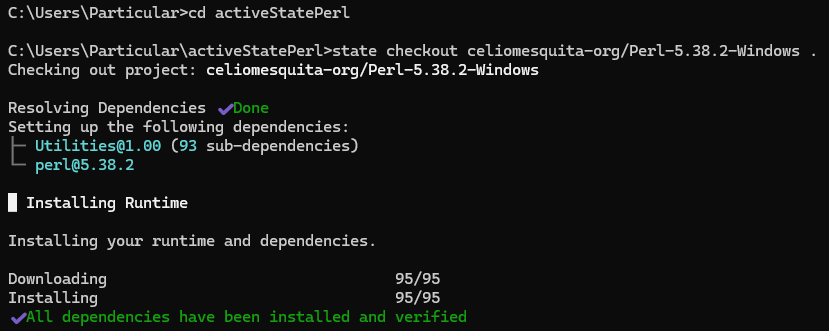
\includegraphics[width=0.95\textwidth]{images/perl_install_1}}
	\caption{Perl instalado com sucesso}
	\label{fig:perl_install_1}
\end{figure}

\begin{figure}[H]
	\centering
	\fbox{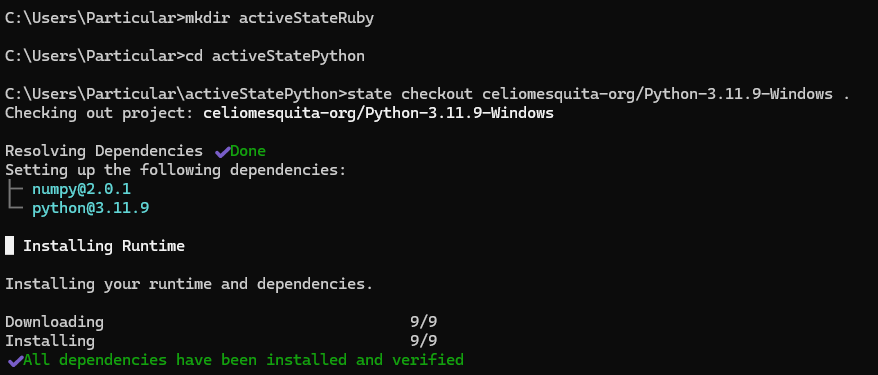
\includegraphics[width=0.95\textwidth]{images/python_install_1}}
	\caption{Python instalado com sucesso.}
	\label{fig:python_install_1}
\end{figure}

\begin{figure}[H]
	\centering
	\fbox{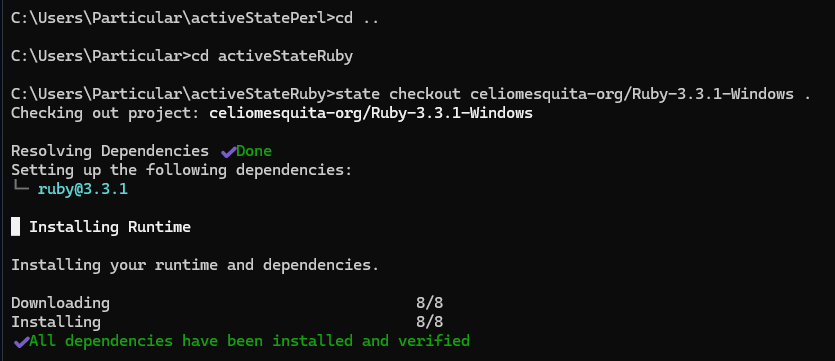
\includegraphics[width=0.95\textwidth]{images/ruby_install_1}}
	\caption{Ruby instalado com sucesso.}
	\label{fig:ruby_install_1}
\end{figure}

\subsubsection{Instalação do compilador C++}
\label{compilador}

Faça o download dos drivers do Microsoft Visual Studio C++ (Visual C++ Redistributable for Visual Studio 2019) do seguinte endereço:

\url{https://learn.microsoft.com/en-us/cpp/windows/latest-supported-vc-redist?view=msvc-160}

Opte pela versão: \url{https://aka.ms/vs/17/release/vc_redist.x64.exe}

\begin{figure}[H]
	\centering
	\fbox{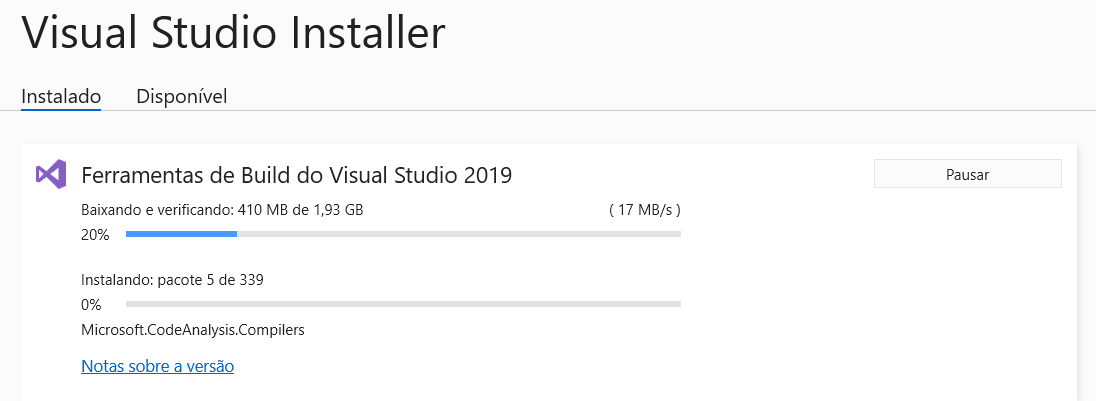
\includegraphics[width=0.95\textwidth]{images/msvc_build_2019}}
	\caption{Visual Studio 2019 versão 16.11.39}\label{fig:msvc_build_2019}
\end{figure}

\cautionbox{\color{purple}A partir deste ponto, todas as compilações serão baseadas em \textbf{Visual Studio 16 2019}.}

\subsubsection{Instalação do \cmake{}}
\label{cmake}

\cmake{} é um sistema para automatizar tarefas de compilação de arquivos de código criados em C e C++. 

\begin{enumerate}
	\item Baixe e instale o \cmake{} por meio do endereço: \url{https://cmake.org/download/}.
	\item Instale a versão \textit{Windows x64 Installer}.
	\item Marque a opção: \textit{Add CMake to the PATH environment variable}.
\end{enumerate}


\subsubsection{Instalando do \textit{Git}}

Acesse o site oficial do Git: \url{https://git-scm.com/download/win}

Selecione esta versão: \textit{64-bit Git for Windows Setup}.

Ao instalar, a não ser que tenha experiência para decidir, utilize todas as opções oferecidas pelo instalador.

Se o Git já estiver instalado, mas ainda não for reconhecido, talvez o caminho (PATH) não tenha sido configurado corretamente.

Adicione o Git ao PATH


\begin{enumerate}

	\item Pressione Win + Pause/Break (Win + I, se for em um notebook) para abrir as Propriedades do Sistema.
	\item Clique em Configurações avançadas do sistema.
	\item Na aba Avançado, clique em Variáveis de Ambiente.
	\item Na seção Variáveis do sistema, localize a variável chamada Path e clique em Editar.
	\item Clique em Novo e adicione o caminho completo para o diretório bin do Git, por exemplo:
	
	\begin{verbatim}
	C:\Program Files\Git\bin
	\end{verbatim}
	
	\item Clique em OK em todas as janelas para salvar as mudanças.

\end{enumerate}


\subsubsection{Construindo o \qtfive{} a partir do \textbf{git}}
\begin{enumerate}
	\item Abra o do terminal \windows{}, copie e cole os seguintes comandos:
	\begin{mdframed}
		\begin{verbatim}
			cd c:\
			git clone git://code.qt.io/qt/qt5.git
			cd qt5
			git checkout 5.15.2 // Compilar exatamente esta versão
		\end{verbatim}
	\end{mdframed}
	
	\item Inicializar os submódulos do repositório (isso pode demorar umas 3h):
	\begin{mdframed}
		\begin{verbatim}
			perl init-repository
		\end{verbatim}
	\end{mdframed}
\end{enumerate}

\cautionbox{
Alterne para o prompt de comando do Desenvolvedor do Visual Studio, a fim de configurar o \qtfive{} para compilação.
}

\cautionbox{\color{orange}
	Ao copiar o comando deste manual, altere-o para ocupar somente uma linha, antes de colar no \textit{Developer Command Prompt}.
	Também pode copiar e uma linha de cada vez, concatenando em uma linha no terminal.
}

Copie e cole o seguinte comando:
\small
\begin{mdframed}
\begin{verbatim}
.\configure.bat -prefix "C:\qt5\Qt5.15.2" -platform win32-msvc2019 release
 -opensource -confirm-license -nomake examples -nomake tests -skip qtwebengine
\end{verbatim}
\end{mdframed}
\normalsize

\newpage

Selecione a opção \textit{Open Source Edition}.
\begin{mdframed}
\begin{verbatim}
Selecting Qt Edition.

Type 'c' if you want to use the Commercial Edition.
Type 'o' if you want to use the Open Source Edition.
\end{verbatim}
\end{mdframed}


A opção {\tt -prefix} no comando {\tt configure.bat} especifica onde o Qt será instalado após o processo de compilação, portanto o diretório {\tt Qt5.15.2} não precisa existir ainda. Ele será criado durante a etapa de instalação (\textit{nmake install}) se ainda não existir.

Agora você pode compilar o \qt{} usando o \textbf{nmake}.
Esta etapa também irá demorar bastante.

\begin{mdframed}
\begin{verbatim}	
	nmake
	nmake install
\end{verbatim}
\end{mdframed}


\subsubsection{Variáveis de ambiente do \qtfive{}}

As variáveis de ambiente permitem que o ambiente de desenvolvimento localize corretamente as bibliotecas do Qt. Elas são especialmente importantes se o Qt foi instalado em um diretório não padrão no \windows{}, como fora de \path{C:\Program Files} ou \path{C:\Program Files (x86)}.

\begin{enumerate}
	\item **Criação da variável QTDIR:**
	\begin{enumerate}
		\item Abra o \textit{Painel de Controle} do \windows{} e navegue até \textit{Sistema e Segurança} > \textit{Sistema} > \textit{Configurações avançadas do sistema}.
		\item Clique em \textit{Variáveis de Ambiente...}.
		\item Na seção \textit{Variáveis de sistema}, clique em \textit{Novo...}.
		\item Crie uma nova variável chamada \textbf{QTDIR}. O valor deve ser o caminho de instalação do \qt{}. Exemplo: \path{C:\Qt\5.15.2\}.
	\end{enumerate}
	
	\begin{figure}[H]\centering
		\fbox{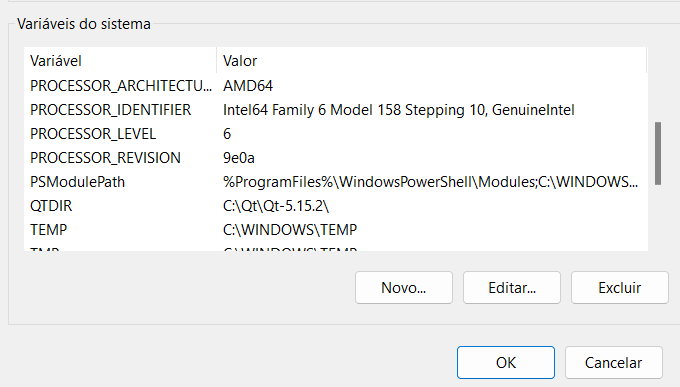
\includegraphics[width=0.75\textwidth]{images/qtdirenv}}
		\caption{Criação da variável de ambiente \emph{QTDIR}}\label{fig:qtdirenv}
	\end{figure}
	
	\item **Atualização da variável Path:**
	\begin{enumerate}
		\item Ainda na tela de variáveis de ambiente, localize e selecione a variável \textbf{Path}, depois clique em \keys{Editar...}.
		\item Na nova tela que se abrirá, clique em \keys{Novo} para adicionar as seguintes entradas à lista existente:
		\begin{mdframed}
		\begin{verbatim}
			%QTDIR%\bin
			%QTDIR%\lib
		\end{verbatim}
		\end{mdframed}
	\end{enumerate}
	
	\begin{figure}[H]\centering
		\fbox{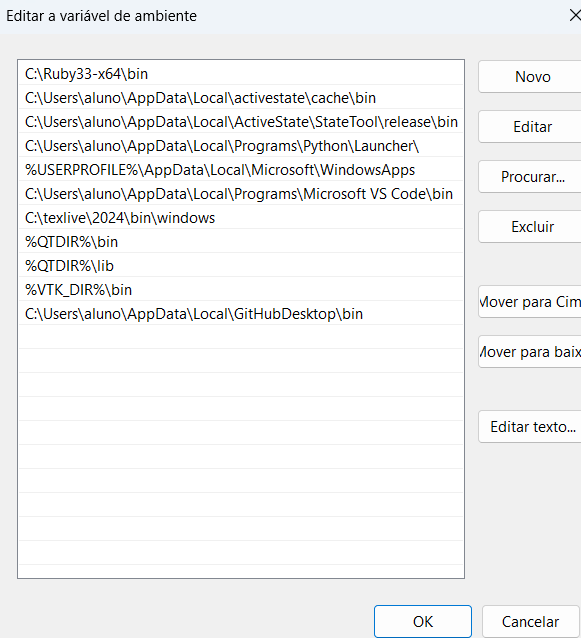
\includegraphics[width=0.75\textwidth]{images/qtpathenv}}
		\caption{Novas variáveis na lista em \emph{Path}}\label{fig:qtpathenv}
	\end{figure}
	
	\item **Reinicialização do sistema:**
	\begin{enumerate}
		\item Faça logout e login ou reinicie o sistema operacional para que as novas variáveis sejam carregadas corretamente.
	\end{enumerate}
\end{enumerate}

Importante ressaltar que, até agora, estivemos instalando somente a infraestrutura.  A seguir virão as ferramentas de desenvolvimento.


\subsection{\textit{Download} e instalação da última versão \textit{Opensource} do \qtcreator{}}

\begin{enumerate}
	\item Acesse a página de \download{} do \qt{} em: \url{https://www.qt.io/download-open-source}
	\item Role a página até atingir a parte de baixo, onde deve visualizar o botão de \download{}.
	\item Clique no botão para iniciar o \download{} do instalador do \qt{} (ver Figura \ref{fig:qtinstallerdown} ).

\begin{figure}[H]
	\centering
	\fbox{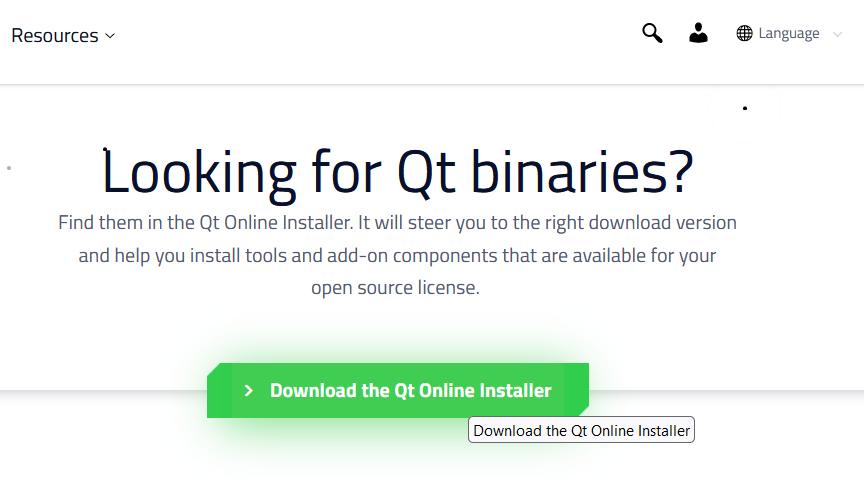
\includegraphics[width=0.75\textwidth]{images/qtinstallerdown}}
	\caption{\download{} do instalador do \qt{} }
	\label{fig:qtinstallerdown}
\end{figure}

\item Também será possível escolher o \textit{mirror}, local de origem do instalador.

\small
\begin{verbatim}
	.\qt-online-installer-windows-x64-4.8.0.exe --mirror https://mirrors.ocf.berkeley.edu/qt/
\end{verbatim}
\normalsize

	\item Na próxima tela, escolha a opção do instalador para sistemas operacionais \windows{} e clique no botão para \download{} (vide Figura \ref{fig:qtinstallerwin}).
	
\begin{figure}[H]
	\centering
	\fbox{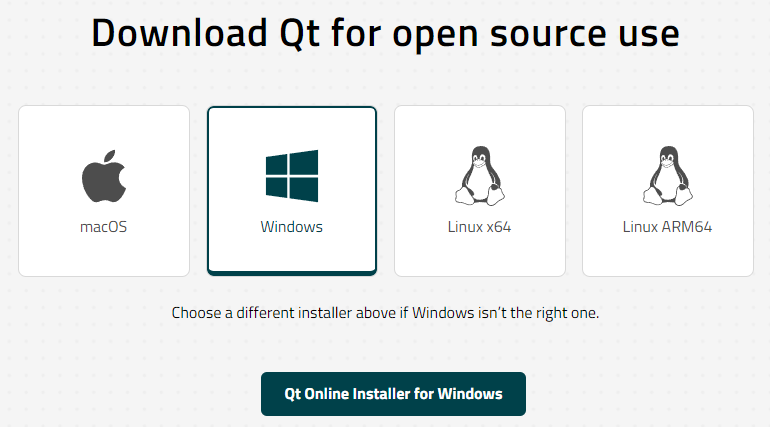
\includegraphics[width=0.75\textwidth]{images/qt_online_installer}}
	\caption{Escolha do instalador por sistema operacional}
	\label{fig:qtinstallerwin}
\end{figure}

\item Na instalação online, a próxima tela oferece a possibilidade de registro de e-mail no ambiente do \qt, conforme a Figura \ref{fig:qt_installer_email}

\begin{figure}[H]
	\centering
	\fbox{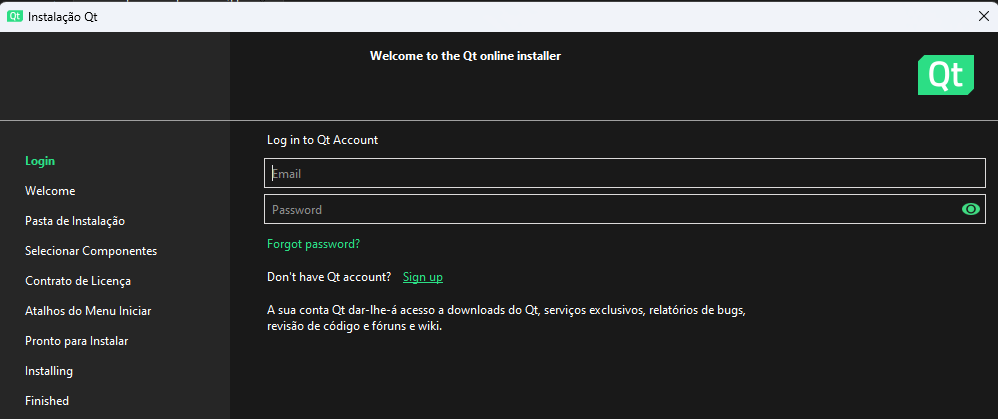
\includegraphics[width=0.95\textwidth]{images/qt_installer_email}}
	\caption{Digite seus dados a fim de continuar o processo de download do \qt{}.}
	\label{fig:qt_installer_email}
\end{figure}

\item Após o registro, será oferecida a possibilidade de concordar com os termos. Marque que concorda e clique em \textbf{Próximo}.

\begin{figure}[H]
	\centering
	\fbox{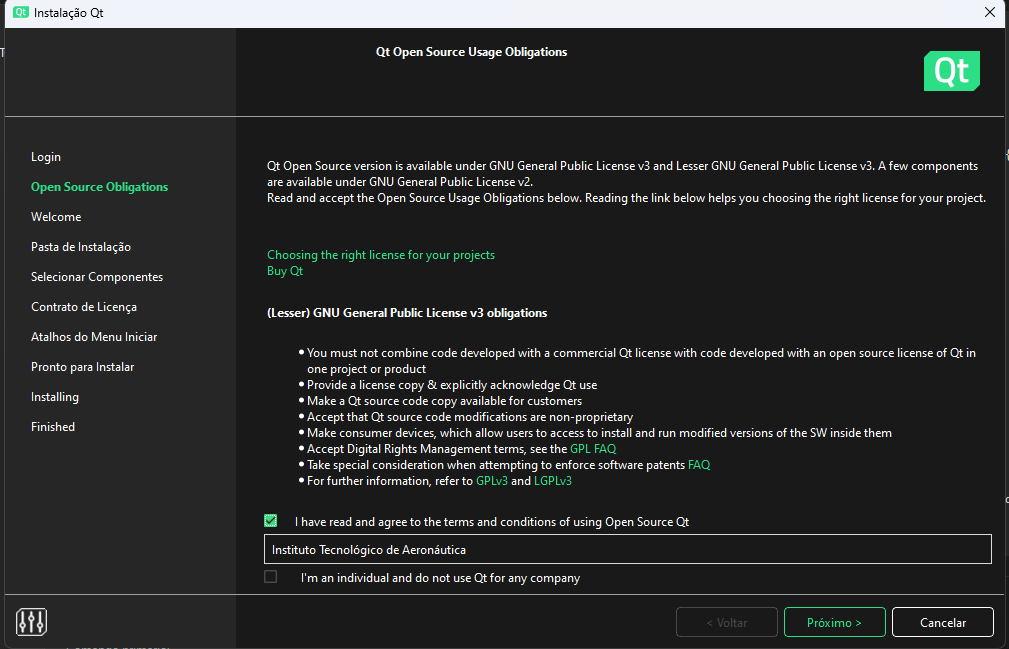
\includegraphics[width=0.95\textwidth]{images/qt_after_email}}
	\caption{ Marque que concorda e clique em \textbf{Próximo}.}
	\label{fig:qt_after_email}
\end{figure}

\item Em seguida, será oferecida a possibilidade de escolher o caminho  para instalação (Figura \ref{fig:qt_download_path}).

\begin{figure}[H]
	\centering
	\fbox{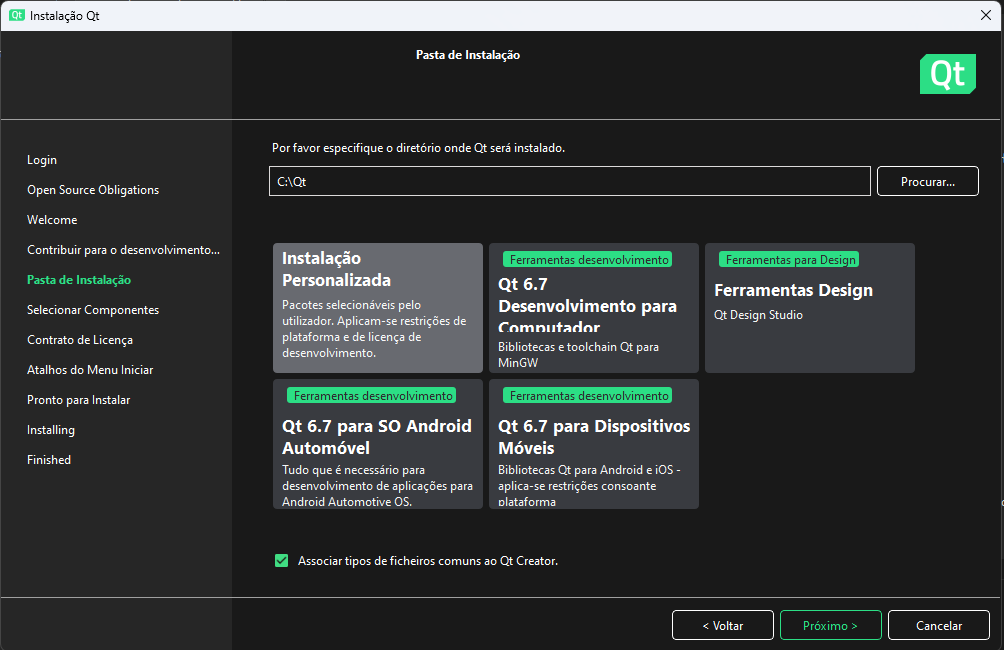
\includegraphics[width=0.95\textwidth]{images/qt_download_path}}
	\caption{ Escolha o caminho e clique em \textbf{Próximo}.}
	\label{fig:qt_download_path}
\end{figure}

\item Em seguida, será oferecida a possibilidade de escolher os componentes da instalação (Figura \ref{fig:qt_inst_modules}). Caso não escolha todos os componentes, poderá instalá-los posteriormente.

\begin{figure}[H]
	\centering
	\fbox{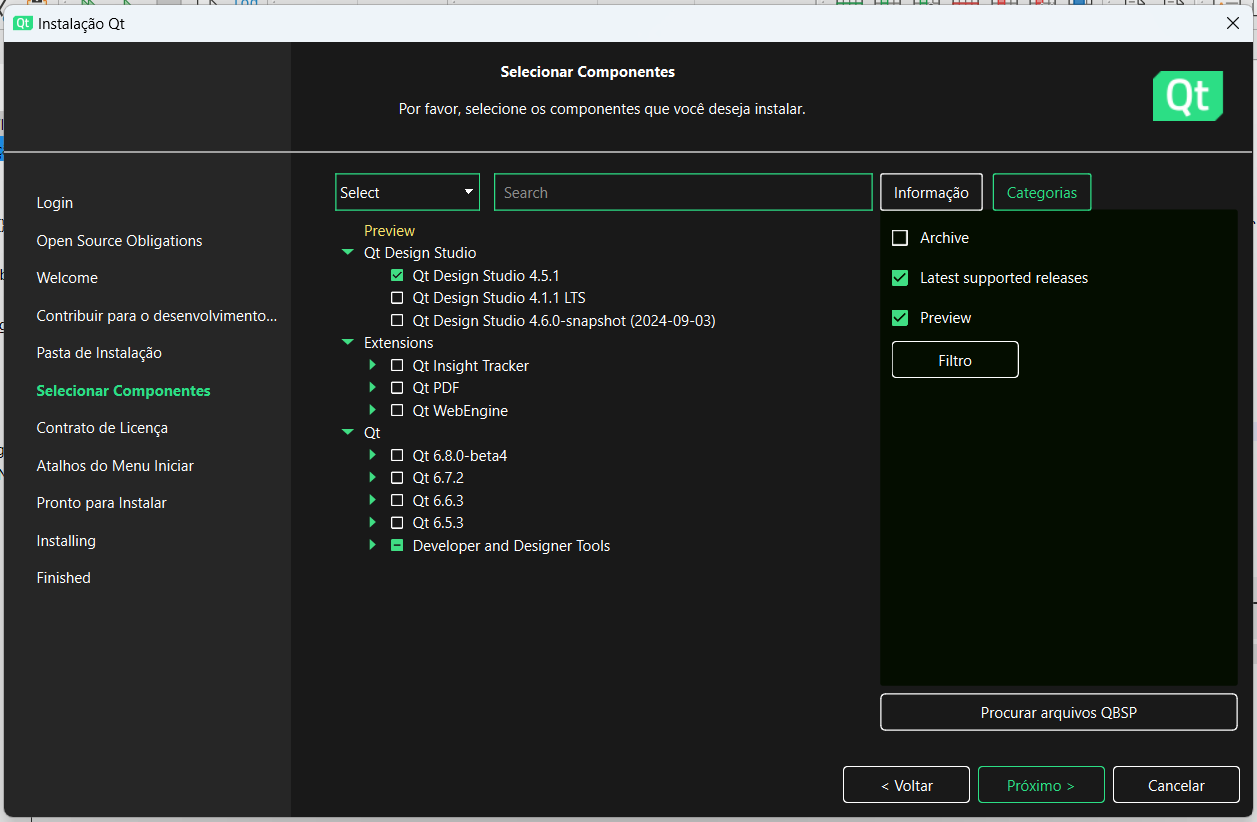
\includegraphics[width=0.95\textwidth]{images/qt_inst_modules}}
	\caption{ Escolha todos os componentes e clique em \textbf{Próximo}.}
	\label{fig:qt_inst_modules}
\end{figure}

Como, no passo anterior (Figura \ref{fig:qt_inst_modules}), não é mais possível optar pelo \qtfive{}, nos restou a opção da instalação a versão \textit{offline}, o que fizemos na subseção \ref{qt5}.

\item Em seguida, será oferecida a possibilidade de marcar que concorda com os termos do \textit{CMake license agreement} (Figura \ref{fig:qt_mark_read}). Marque e continue com o processo de instalação.

\begin{figure}[H]
	\centering
	\fbox{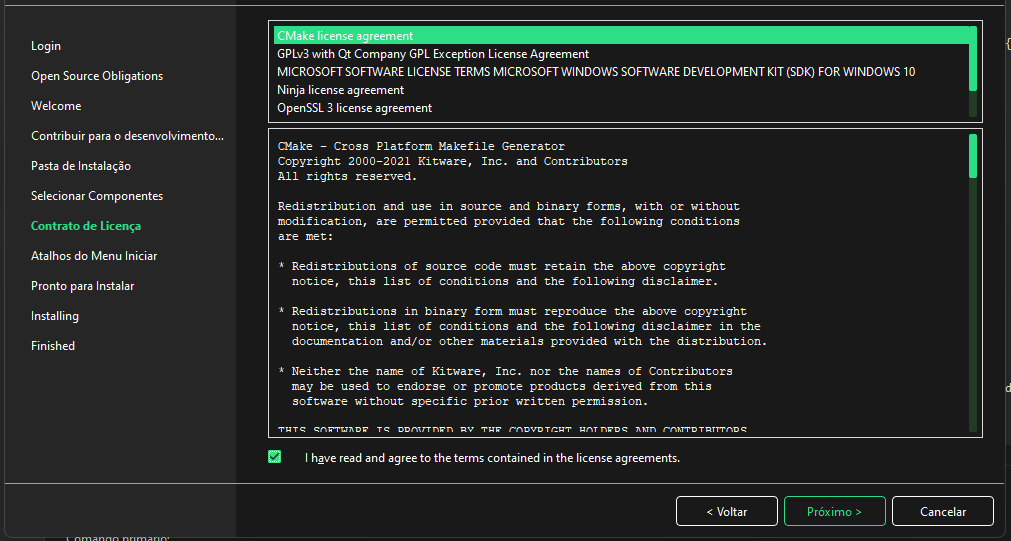
\includegraphics[width=0.95\textwidth]{images/qt_mark_read}}
	\caption{ Marque que concorda e clique em \textbf{Próximo}.}
	\label{fig:qt_mark_read}
\end{figure}

\item Aguarde a conclusão da instalação (Figura \ref{fig:qt_wait_inst_finish}).

\begin{figure}[H]
	\centering
	\fbox{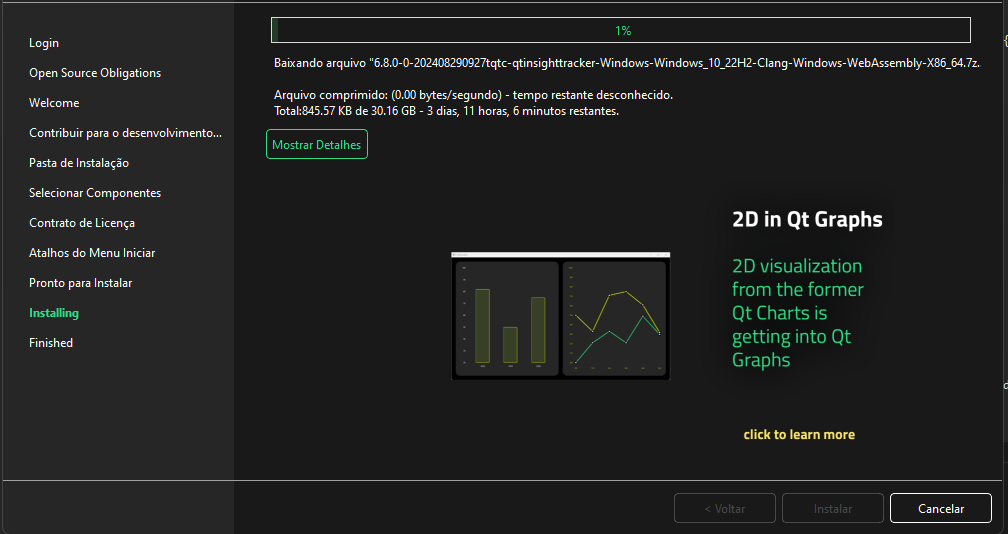
\includegraphics[width=0.95\textwidth]{images/qt_wait_inst_finish}}
	\caption{Andamento da instalação do \qtcreator{}.}
	\label{fig:qt_wait_inst_finish}
\end{figure}

\end{enumerate}



\subsection{Instalação do \visualstudio{}}

\cautionbox{\color{blue}Não é necessário instalar o \visualstudio{}, a não ser que você tenha habilidade no seu uso e não queira utilizar o \qtcreator{}.
Com relação aos drivers de C++, já o fizemos na subseção \ref{compilador}.
 }

O \visualstudio{} é uma IDE desenvolvida e mantida pela \textit{Microsoft}, amplamente utilizada em sistemas operacionais \windows{}. Ele utiliza o compilador \emph{Microsoft Visual C++} (\msvc{}), uma alternativa ao \emph{GNU Compiler Collection} (GCC) mais comum em ambientes \linux{}. Neste projeto, poderemos utilizar a versão 2019 do \visualstudio{} e do compilador \msvc{}.

\begin{enumerate}

\item No \qtcreator{} ou no \vscode{}, configure o compilador compatível com o Qt 5.15.2, agora disponíveis após a instalação das ferramentas de \textit{Build}.

\begin{figure}[H]
	\centering
	\fbox{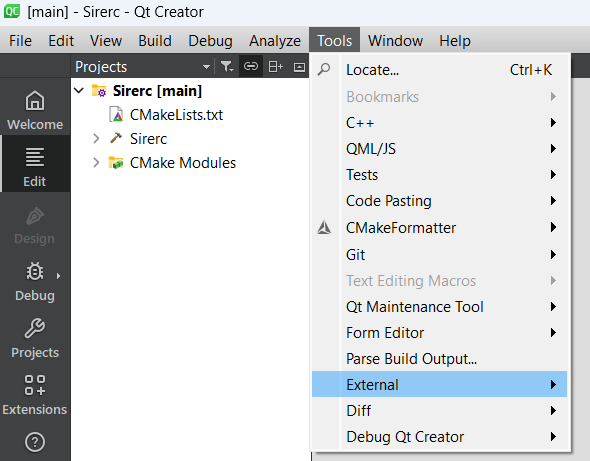
\includegraphics[width=0.75\textwidth]{images/qt_tools_ext_config}}
	\caption{Configurar o \qtcreator{} para build}\label{fig:qt_tools_ext_config}
\end{figure}

\item Escolha o kit de compilação baixado, o Visual Studio 2019 version 16.11.3, o Microsoft Visual C++ compiler, versão 16.11.x

\begin{figure}[H]
	\centering
	\fbox{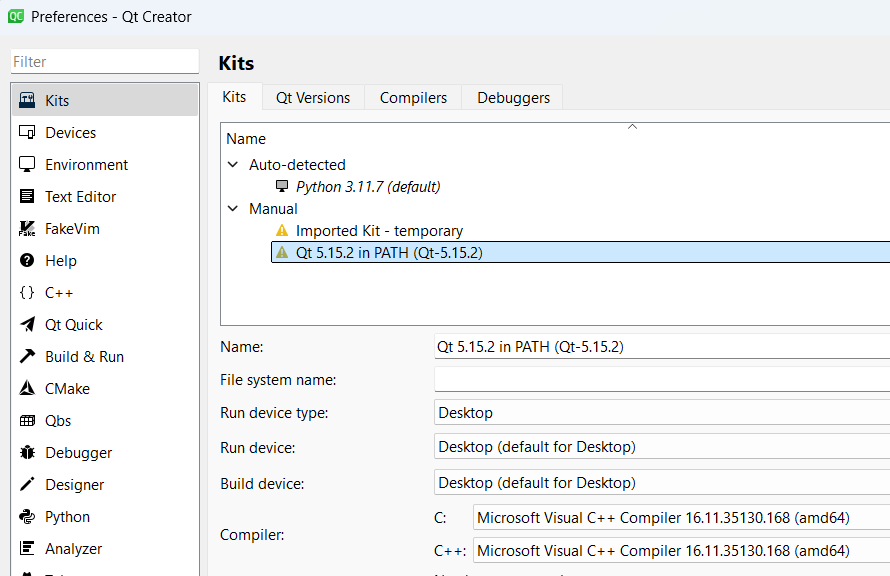
\includegraphics[width=0.95\textwidth]{images/qt_tools_ext_config_kit}}
	\caption{Escolha o kit de compilação baixado.}\label{fig:qt_tools_ext_config_kit}
\end{figure}

\begin{figure}[H]
	\centering
	\fbox{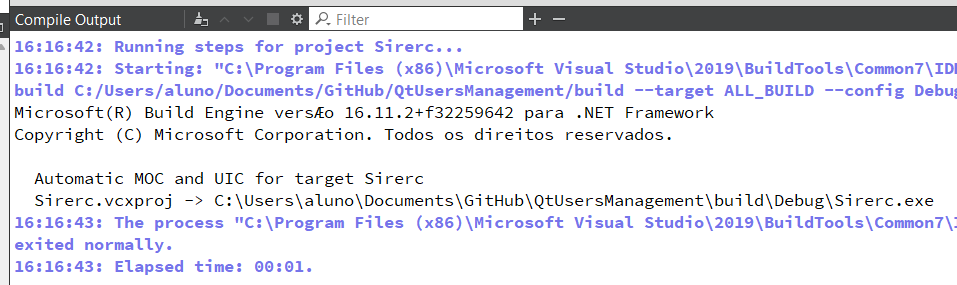
\includegraphics[width=0.95\textwidth]{images/qt_no_error_compile}}
	\caption{Compilação realizada sem erros.}\label{fig:qt_no_error_compile}
\end{figure}

\end{enumerate}


\subsection{Instalação do \mongo{}}

\cautionbox{\color{red}"Sub judice"}

\color{brown}

Com a finalidade de controlar os projetos dos usuários do \sistema{}, poderemos utilizar o banco de dados não relacional \mongo{}, que armazena as informações no formato de objetos \textbf{json}.

Isto tem potencial de contribuir para a segurança dos dados industriais.

Baixe e instale o \mongo{} a partir do endereço: \url{https://www.mongodb.com/try/download/community}.

\begin{figure}[H]
	\centering
	\fbox{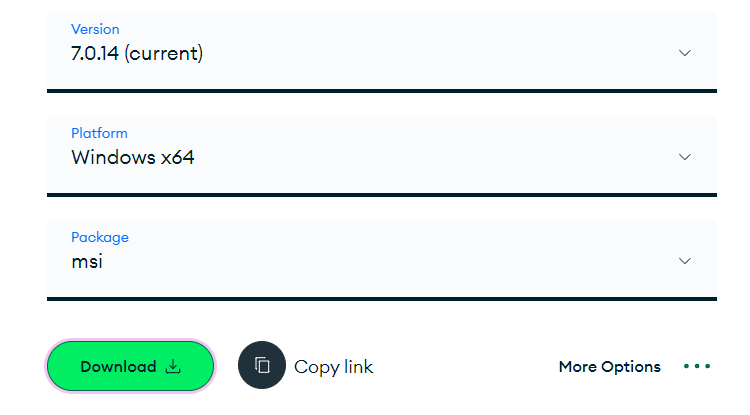
\includegraphics[width=0.65\textwidth]{images/mongodb_download_2}}
	\caption{Clique em \download{}.}\label{fig:mongodb_download_2}
\end{figure}

Clique na opção \textit{Complete} e continue a instalação.

Agora com o \mongo{} instalado, vamos instalar os drivers de C++ para \mongo{}, a serem utilizados pelo \qtcreator{}.


\subsubsection{Drivers de C++ para \mongo{}}

Baixe a versão mais recente do driver \textbf{mongocxx}
O ponto de partida mais confiável para criar o driver \textbf{mongocxx} é o \textit{tarball} (arquivo compactado) da versão mais recente.

Os lançamentos do \textbf{mongocxx} terá links para o \textit{tarball} de versão da versão que você deseja instalar.

\cautionbox{\color{orange}Comandos deste manual grafados em mais de uma linha, precisam ser editados para somente uma linha, antes de colar no terminal.}

Baixe e descompacte do endereço: \url{https://github.com/mongodb/mongo-cxx-driver/releases/tag/r3.10.2}

Abra o \textit{Developer Command Prompt}.
\begin{mdframed}
\begin{verbatim}
cd C:/Users/<seu usuário>/Downloads/
\end{verbatim}
\end{mdframed}

\subsubsection{Configurar o driver}

\begin{mdframed}
	\begin{verbatim}
	cd mongo-cxx-driver-r3.10.2/mongo-cxx-driver-r3.10.2
	cmake -G "Visual Studio 16 2019" -A x64 -DCMAKE_CXX_STANDARD=17
	 -DCMAKE_BUILD_TYPE=Release
	\end{verbatim}
\end{mdframed}

Caso o comando \textbf{cmake} não seja reconhecido, coloque este endereço no \textbf{path}

{\tt C:/Program Files/CMake/bin} e repita os comandos acima.

\subsubsection{Compilar o driver}

Agora que os arquivos de build foram gerados, você pode iniciar a compilação do driver. No Prompt de Comando do Desenvolvedor do Visual Studio ou no terminal que você está usando, execute o seguinte comando para compilar o projeto:

\begin{mdframed}
	\begin{verbatim}
	cmake --build . --config Release
	\end{verbatim}
\end{mdframed}

Esse comando compilará o driver no modo Release. Como pode ser bastante demorado, você pode, antes de iniciar, tentar conseguir uma versão já compilada de algum colega.

\subsubsection{Instalar o driver}

Crie a pasta {\tt Drivers} no seu computador, se não existir.

Execute o seguinte comando para instalar o driver:
\begin{mdframed}
	\begin{verbatim}
cmake --install . --config Release --prefix "C:/Drivers/mongo-cxx-driver"
	\end{verbatim}
\end{mdframed}

Agora os arquivos devem estar corretamente instalados no diretório {\tt C:/Drivers/mongo-cxx-driver}. A partir daqui, você pode usar o \textbf{mongo-cxx-driver} em seus projetos C++ vinculando as bibliotecas e incluindo os cabeçalhos instalados.

\begin{figure}[H]
	\centering
	\fbox{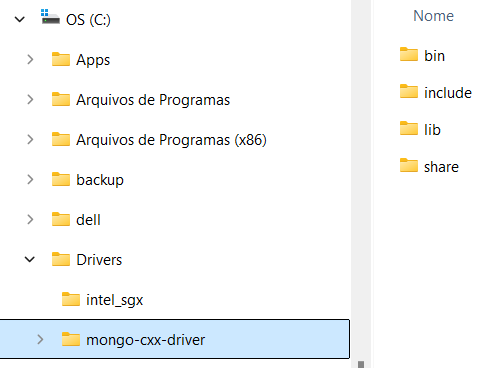
\includegraphics[width=0.55\textwidth]{images/mongodb_drivers}}
	\caption{Drivers de C++ para \mongo{} instalados com sucesso.}\label{fig:mongodb_drivers}
\end{figure}

\subsubsection{Criação de objetos no \mongo{}}

O \mongo{} vem com uma ferramenta para administração de objetos \textbf{json}, o \textit{Compass}.
\begin{figure}[H]
	\centering
	\fbox{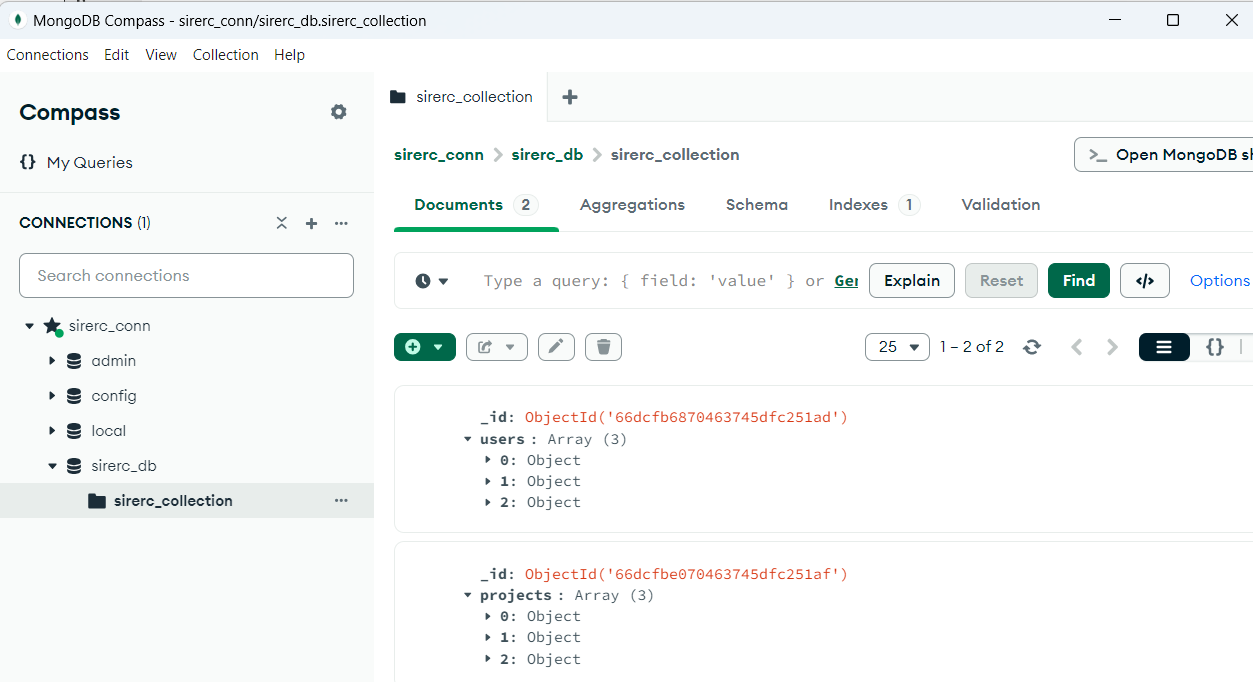
\includegraphics[width=0.95\textwidth]{images/mongo_compass}}
	\caption{\mongo{} Compass}\label{fig:mongo_compass}
\end{figure}

Na Figura \ref{fig:mongo_compass}, pode-se observar que foram criados os objetos:
\begin{enumerate}
\item sirerc\_conn
\item sirerc\_db
\item sirerc\_collection
\end{enumerate}

No $sirerc\_collection$, criamos duas coleções: $users$ e $projects$.

A coleção $users$ será utilizada para associar usuários e seus projetos. A coleção $projects$ será utilizada para registrar os projetos e suas informações. 

\color{black}

\newpage
\subsection{Instalação do VTK}
\label{vtk}

O \emph{Visualization Toolkit} (VTK) é um software multiplataforma utilizado para computação gráfica 3D, visualização e processamento de imagens. No \sistema{}, o VTK é usado para visualizar os resultados gráficos após a execução do simulador, relacionados ao problema de dinâmica de fluidos.

\begin{enumerate}
	\item Baixe o código-fonte da versão 9.3.0 RC1 do VTK, atualmente em uso no \sistema{}, no seguinte endereço: \url{https://gitlab.kitware.com/vtk/vtk/-/archive/v9.3.0.rc1/vtk-v9.3.0.rc1.zip}.
	\item Descompacte no diretório Downloads.
	
	\begin{enumerate}
	\item 	Caso deseje, você pode descompactar com o botão direito do mouse sobre o arquivo \textbf{.zip} ou \textbf{.tar.gz}.
	\item 	Também é possível, em um terminal do \windows{}, digitar WSL, acessando o terminal do \linux{}, e colar este comando: {\tt tar -xvf vtk-v9.3.0.rc1.zip}.
	\end{enumerate}
	
	\item Abra o \textit{Developer Command Prompt}.
\end{enumerate}


\subsubsection{Configurar o driver}

Na extração, serão criados dois diretórios: {\tt vtk-v9.3.0.rc1/vtk-v9.3.0.rc}

\begin{mdframed}
	\begin{verbatim}
		cd Downloads/vtk-v9.3.0.rc1/vtk-v9.3.0.rc1
		mkir build
		cd build
		
		cmake -G "Visual Studio 16 2019" -A x64 -DCMAKE_CXX_STANDARD=17
		 -DCMAKE_BUILD_TYPE=Release ..
	\end{verbatim}
\end{mdframed}

Os dois pontos no final fazem com que o comando se refira ao diretório pai.

Caso o comando \textbf{cmake} não seja reconhecido, coloque este endereço no \textbf{path}

{\tt C:/Program Files/CMake/bin} e repita o \cmake{} acima.

\begin{figure}[H]
	\centering
	\fbox{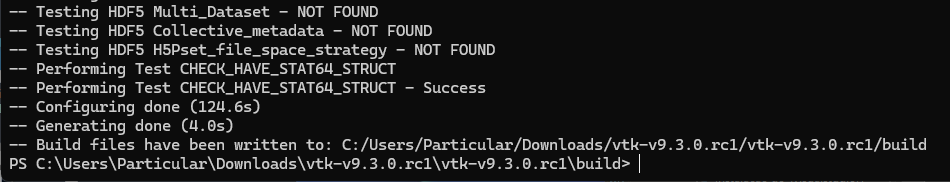
\includegraphics[width=0.95\textwidth]{images/vtk_make}}
	\caption{VTK drivers configurados para o Visual Studio 16 2019 com sucesso.}
	\label{fig:vtk_make}
\end{figure}

\subsubsection{Compilar o driver}

Agora que os arquivos de \textit{build} foram gerados, você pode iniciar a compilação do VTK. Execute o seguinte comando para compilar o projeto:
\begin{mdframed}
	\begin{verbatim}
	cmake --build . --config Release 
	\end{verbatim}
\end{mdframed}

Esse comando compilará o \textit{driver} no modo \textit{Release}, que depois será instalado em {\tt C:/Drivers/VTK}.

\subsubsection{Instalar o driver}

\begin{enumerate}
	\item Crie a pasta {\tt Drivers} no seu computador, se não existir.
	\item Execute o seguinte comando para instalar o driver:
	
	\begin{mdframed}
		\begin{verbatim}
			cmake --install . --config Release --prefix "C:\Drivers\VTK"
		\end{verbatim}
	\end{mdframed}
\end{enumerate}

\begin{figure}[H]
	\centering
	\fbox{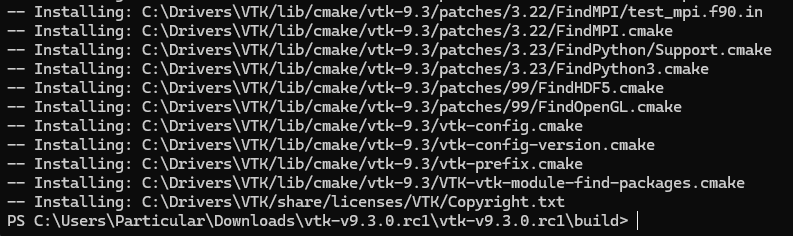
\includegraphics[width=0.95\textwidth]{images/vtk_drivers}}
	\caption{VTK drivers gerados com sucesso.}
	\label{fig:vtk_drivers}
\end{figure}

\subsubsection{Variáveis de Ambiente do VTK}

\begin{enumerate}
	\item **Criação da variável VTK\_DIR:**
	\begin{enumerate}
		\item Abra o \textit{Painel de Controle} do \windows{} e navegue até \textit{Sistema e Segurança} > \textit{Sistema} > \textit{Configurações avançadas do sistema}.
		\item Clique em \textit{Variáveis de Ambiente...}.
		\item Na seção \textit{Variáveis de sistema}, clique em \textit{Novo...}.
		\item Crie uma nova variável chamada \textbf{VTK\_DIR}. O valor deve ser o caminho do diretório onde o VTK foi instalado. 
	\end{enumerate}
	
	\item **Atualização da variável Path:**
	\begin{enumerate}
		\item Ainda na tela de variáveis de ambiente, localize e selecione a variável \textbf{Path}, depois clique em \keys{Editar...}.
		\item Na nova tela que se abrirá, clique em \keys{Novo} para adicionar a seguinte entrada à lista existente:
		\begin{mdframed}
		\begin{verbatim}
			%VTK_DIR%\bin
		\end{verbatim}
		\end{mdframed}
	\end{enumerate}
	
	\item **Reinicialização do sistema:**
	\begin{enumerate}
		\item Faça logout e login ou reinicie o sistema para que as novas variáveis sejam carregadas corretamente.
	\end{enumerate}
\end{enumerate}

\newpage
\subsection{Instalação do \gmsh{}}

O \gmsh{} é um gerador de malha de elementos finitos 3D de código aberto, com um mecanismo CAD integrado e pós-processador. No \sistema{}, o \gmsh{} é utilizado para gerar a malha que representa o domínio a ser simulado, como poços de petróleo.

Seu objetivo de design é fornecer uma ferramenta de malha rápida, leve e fácil de usar com entrada paramétrica e recursos avançados de visualização. O \gmsh{} é construído em torno de quatro módulos: geometria, malha, solucionador e pós-processamento. A especificação de qualquer entrada para esses módulos é feita interativamente usando a interface gráfica do usuário ou em arquivos de texto ASCII usando a própria linguagem de \textit{script} do \gmsh{}.

\begin{enumerate}
	\item Baixe o código-fonte da versão 4.11.1 do \gmsh{}, atualmente em uso no \sistema{}, no seguinte endereço: \url{https://gmsh.info/src/gmsh-4.11.1-source.tgzp}.
	\item Descompacte no diretório Downloads.
	\item Abra o \textit{Developer Command Prompt}.
\end{enumerate}

\subsubsection{Configurar o driver}

Na extração, serão criados dois diretórios: {\tt vtk-v9.3.0.rc1/vtk-v9.3.0.rc}

\begin{mdframed}
	\begin{verbatim}
		cd Downloads\gmsh-4.11.1-source\gmsh-4.11.1-source
		mkir build
		cd build
		

cmake -G "Visual Studio 16 2019" -A x64 -DCMAKE_CXX_STANDARD=17 -DCMAKE_BUILD_TYPE=Release
 -DENABLE_OPENMP=False
  -DENABLE_PRIVATE_API=True
   -DENABLE_BUILD_DYNAMIC=True
    -DENABLE_TESTS=False
		
	\end{verbatim}
\end{mdframed}


\begin{figure}[H]
	\centering
	\fbox{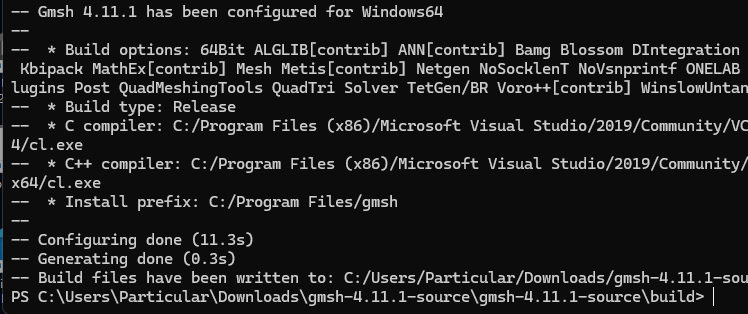
\includegraphics[width=0.95\textwidth]{images/gmsh_build}}
	\caption{\gmsh{} drivers configurados para o Visual Studio 16 2019 com sucesso.}
	\label{fig:gmsh_build}
\end{figure}

\subsubsection{Compilar o driver}

Agora que os arquivos de \textit{build} foram gerados, você pode iniciar a compilação do \gmsh{}. Execute o seguinte comando para compilar o projeto:
\begin{mdframed}
	\begin{verbatim}
		cmake --build . --config Release 
	\end{verbatim}
\end{mdframed}

Esse comando compilará o \textit{driver} no modo \textit{Release}, que depois será instalado em {\tt C:/Drivers/Gmsh}.

\subsubsection{Instalar o driver}

\begin{enumerate}
	\item Execute o seguinte comando para instalar o driver:
	\begin{mdframed}
		\begin{verbatim}
			cmake --install . --config Release --prefix "C:\Drivers\Gmsh"
		\end{verbatim}
	\end{mdframed}
\end{enumerate}

\begin{figure}[H]
	\centering
	\fbox{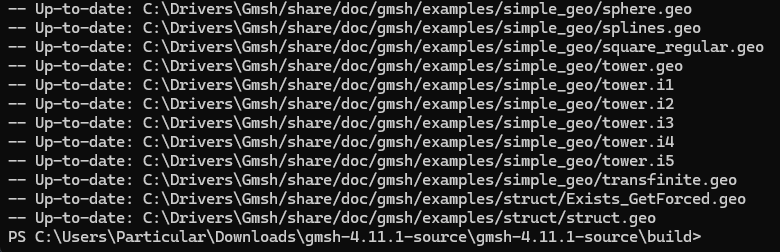
\includegraphics[width=0.95\textwidth]{images/gmsh_install}}
	\caption{\gmsh{} drivers instalados com sucesso em {\tt C:/Drivers/Gmsh}.}
	\label{fig:gmsh_install}
\end{figure}


\subsubsection{Variáveis de Ambiente do \gmsh{}}

	\begin{enumerate}
		\item Tecle Win + I para acessar as configurações do \windows{} e localize $variáveis\ de\ ambiente$.
		\item Na seção \textit{Variáveis de sistema}, clique em \textit{Novo...}.
		\item Crie uma nova variável chamada $GMSH\_INC$. O valor deve ser o caminho dos drivers do GMSH. Exemplo: \path{C:\Drivers\Gmsh\include}.
		\item Em seguida, crie outra variável chamada $GMSH\_LIB$. Exemplo: \path{C:\Drivers\Gmsh\lib}.
	\end{enumerate}
	
\begin{figure}[H]
	\centering
	\fbox{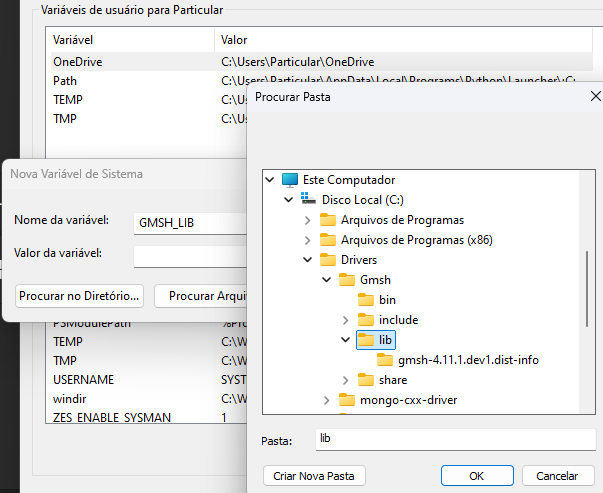
\includegraphics[width=0.85\textwidth]{images/gmsh_lib}}
	\caption{Configuração da variável $GMSH\_LIB$.}
	\label{fig:gmsh_lib}
\end{figure}
	
Faça logout e login ou reinicie o sistema para que as novas variáveis sejam carregadas corretamente.

\subsection{Compilação do \sistema{}}

Neste ponto, o ambiente está pronto para compilar o código do \sistema{}. Este guia foi testado com a versão do sistema disponível na branch \emph{development} do projeto no GitHub em 25/04/2024.

\begin{enumerate}
	\item **Clonando o repositório:**
	\begin{enumerate}
		\item Faça o \emph{clone} do repositório Git disponível em \url{https://github.com/sirercita/SIRERC_ProjetoPetrobras} usando a ferramenta de sua preferência, como \textit{Sourcetree} ou \textit{Git Bash}.
	\end{enumerate}
	
	\item **Checkout do commit de referência:**
	\begin{enumerate}
		\item Faça o \emph{checkout} do \emph{commit} de referência usando a ferramenta de sua preferência. O \emph{hash} do \emph{commit} de referência é \texttt{3f635a7}.
	\end{enumerate}
	
	\item **Preparação do diretório:**
	\begin{enumerate}
		\item Navegue até o diretório do \sistema{} no sistema de arquivos e, na pasta principal, exclua definitivamente todos os diretórios cujo nome inicie com \path{build-}. Esses diretórios são gerados automaticamente pelo \qtcreator{}.
		\item Ainda no diretório do \sistema{}, remova o arquivo \path{FonteSirerc\CMakeLists.txt.user}. Esse arquivo é gerado automaticamente pelo \qtcreator{} e depende da instalação de cada usuário.
	\end{enumerate}
	
	\item **Configuração no \qtcreator{}:**
	\begin{enumerate}
		\item Inicie o \qtcreator{}, a IDE instalada durante a configuração do Qt. Na tela inicial, selecione a versão 5.15.2 do Qt (vide Figura \ref{fig:qtcreatorver}).
		
		\begin{figure}[H]\centering
			\fbox{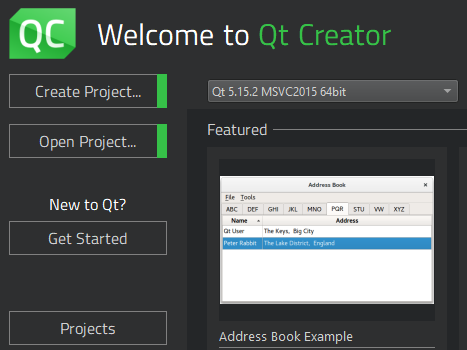
\includegraphics[width=0.75\textwidth]{images/qtcreatorver.png}}
			\caption{Tela inicial do \qtcreator{} e escolha de versão}\label{fig:qtcreatorver}
		\end{figure}
		
		\item Clique no botão 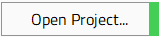
\includegraphics[height=1.5em]{images/qtcreatoropen.png}, navegue até o diretório onde está o código do \sistema{} e selecione o arquivo \path{FonteSirerc/CMakeLists.txt} para abrir o projeto.
		
		\item Ao abrir o projeto, o \qtcreator{} pode exibir um alerta relacionado às configurações locais que precisam ser refeitas automaticamente (vide Figura \ref{fig:qtcreatoralert}). Esse alerta pode ser ignorado clicando em \keys{OK}. Ele aparecerá apenas uma vez.
		
		\begin{figure}[H]\centering
			\fbox{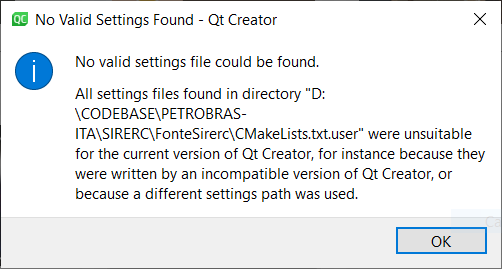
\includegraphics[width=0.55\textwidth]{images/qtcreatoralert.png}}
			\caption{Alerta de primeira utilização do \qtcreator{}}\label{fig:qtcreatoralert}
		\end{figure}
		
		\item Na tela seguinte, o \qtcreator{} solicitará que você selecione os compiladores e arquiteturas a serem suportados no projeto. Mantenha selecionada apenas a versão com o compilador \msvc{}2015 64-bit (vide Figura \ref{fig:qtcreatorconf}) e clique em \keys{Configure Project} na parte inferior da tela.
		
		\begin{figure}[H]\centering
			\fbox{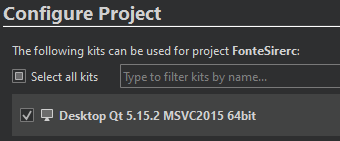
\includegraphics[width=0.55\textwidth]{images/qtcreatorconf.png}}
			\caption{Seleção do tipo de compilador e plataforma no \qtcreator{}}\label{fig:qtcreatorconf}
		\end{figure}
	\end{enumerate}
	
	\item **Configuração do projeto:**
	\begin{enumerate}
		\item Aguarde o \qtcreator{} finalizar o carregamento do projeto. Se tudo estiver correto, você verá a árvore de diretórios do projeto (vide Figura \ref{fig:qtcreatorsirerc}). Se houver algum problema, verifique se o campo \emph{Build Directory} aponta para a pasta \path{build-FonteSirerc-Desktop_Qt_5_15_2_\msvc{}2015_64bit-Release} correta. Modifique-o se necessário e, em seguida, clique na aba \emph{Initial Configuration} e reconfigure o projeto clicando em \emph{Re-configure with Initial Parameters}.
		
		\begin{figure}[H]\centering
			\fbox{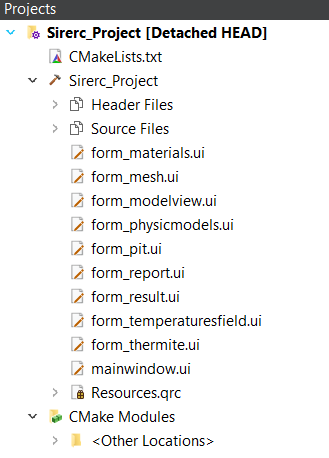
\includegraphics[width=0.35\textwidth]{images/qtcreatorsirerc.png}}
			\caption{Árvore de diretórios do \sistema{}}\label{fig:qtcreatorsirerc}
		\end{figure}
		
		\item Na parte inferior esquerda do \qtcreator{}, altere o tipo de \build{} de \emph{Debug} para \emph{Release} e aguarde a reconfiguração (vide Figura \ref{fig:qtcreatorrelease}).
		
		\begin{figure}[H]\centering
			\fbox{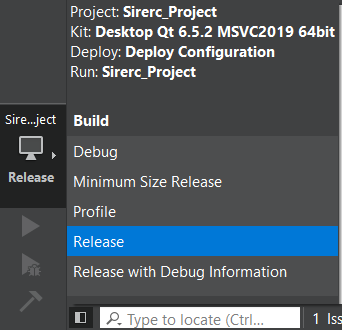
\includegraphics[width=0.45\textwidth]{images/qtcreatorrelease.png}}
			\caption{Mudança de \build{} para \emph{Release} no \qtcreator{}}\label{fig:qtcreatorrelease}
		\end{figure}
	\end{enumerate}
	
	\item **Execução do \sistema{}:**
	\begin{enumerate}
		\item Neste ponto, o \sistema{} pode ser executado clicando no botão 
\includegraphics[height=1.5em]{images/sirercrun.png} no \qtcreator{}. A tela principal do \sistema{} deverá ser exibida após alguns segundos de inicialização (vide Figura \ref{fig:sirerc}).
		
		\begin{figure}[H]\centering
			\fbox{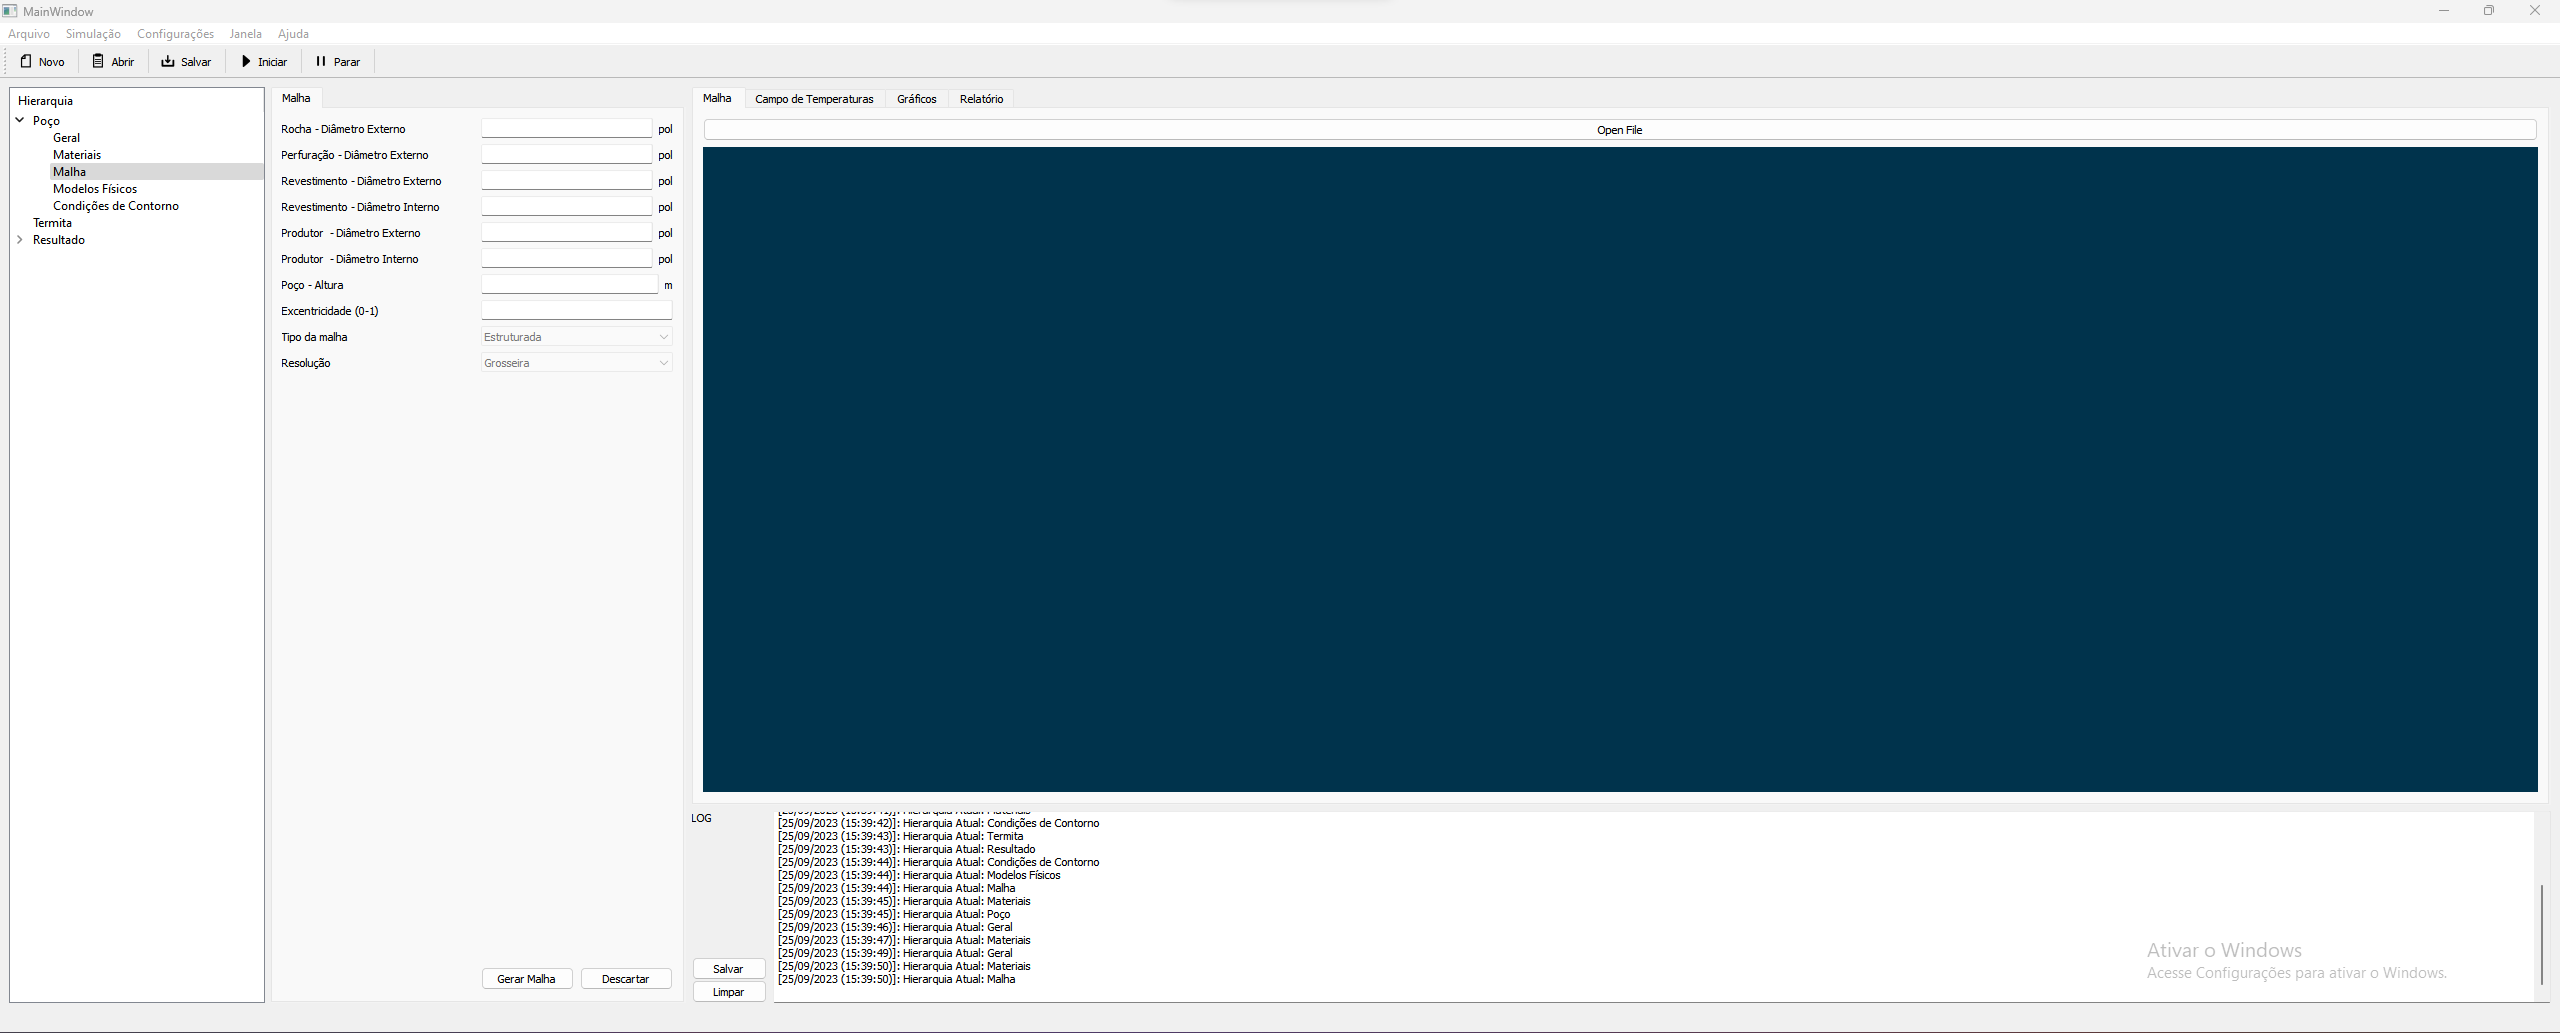
\includegraphics[width=0.95\textwidth]{images/sirerc.png}}
			\caption{\sistema{} em execução}\label{fig:sirerc}
		\end{figure}
	\end{enumerate}
\end{enumerate}

\subsection{Criação do Instalador}

Um instalador \emph{offline} simplifica o processo de instalação ao fornecer uma interface amigável e incluir todas as dependências necessárias em um único arquivo. Projetos baseados no Qt, como o \sistema{}, podem utilizar o módulo QtInstallerFramework para gerar instaladores multiplataforma.

\begin{enumerate}
	\item **Instalação do QtInstallerFramework:**
	\begin{enumerate}
		\item O QtInstallerFramework está disponível como um componente opcional durante a instalação inicial do Qt ou pode ser instalado posteriormente usando a ferramenta QtMaintenanceTool. Em ambos os casos, selecione o módulo na lista de componentes disponíveis e prossiga com a instalação (vide Figura \ref{fig:qtinstallerframework}).
		
		\begin{figure}[H]\centering
			\fbox{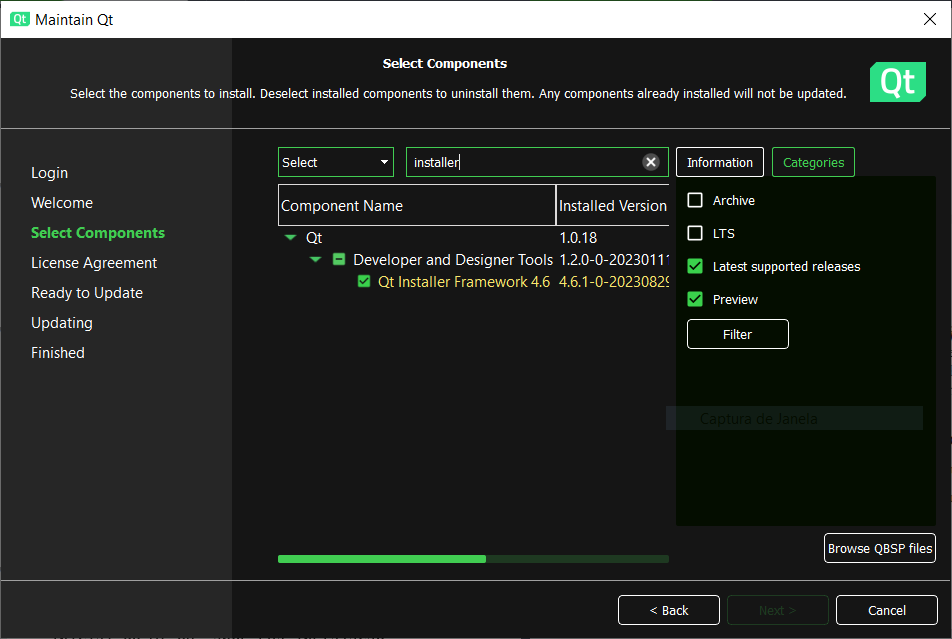
\includegraphics[width=0.7\textwidth]{images/qtinstallerframework.png}}
			\caption{Instalação do componente QtInstallerFramework}\label{fig:qtinstallerframework}
		\end{figure}
	\end{enumerate}
	
	\item **Preparação do ambiente de deployment:**
	\begin{enumerate}
		\item Após a instalação, o QtInstallerFramework estará disponível no diretório \path{${QtDirectory}/Tools/QtInstallerFramework}, onde \path{${QtDirectory}} representa o caminho do sistema de arquivos onde o Qt está instalado.
		\item Crie um diretório temporário em qualquer local do sistema de arquivos para preparar o \sistema{} para \emph{deployment}.
		\item Dentro deste diretório, crie dois subdiretórios chamados \path{config} e \path{packages}, ambos inicialmente vazios (vide Figura \ref{fig:sirercinstallerdir}).
		
		\begin{figure}[H]\centering
			\fbox{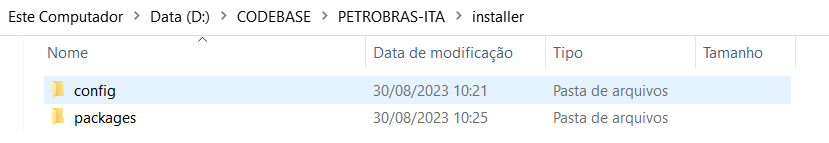
\includegraphics[width=0.75\textwidth]{images/sirercinstallerdir.png}}
			\caption{Diretório inicial para geração do instalador}\label{fig:sirercinstallerdir}
		\end{figure}
	\end{enumerate}
	
	\item **Configuração do arquivo config.xml:**
	\begin{enumerate}
		\item No diretório \path{config}, crie um arquivo chamado \path{config.xml} com o seguinte conteúdo:
		
		\begin{lstlisting}
			<?xml version="1.0" encoding="UTF-8"?>
			<Installer>
			<Name>SIRERC</Name>
			<Version>1.0.0</Version>
			<Title>SIRERC Installer</Title>
			<Publisher>ITA</Publisher>
			<StartMenuDir>SIRERC</StartMenuDir>
			<TargetDir>@HomeDir@/SIRERC</TargetDir>
			</Installer>
		\end{lstlisting}
		
		\item Verifique as \emph{tags} aceitas neste arquivo na documentação do Qt em \url{https://doc.qt.io/qtinstallerframework/ifw-globalconfig.html}. O conteúdo apresentado é apenas um exemplo; verifique se há uma versão mais completa deste arquivo em uso no \sistema{}.
	\end{enumerate}
	
	\item **Configuração dos pacotes:**
	\begin{enumerate}
		\item Um \emph{package} é um módulo que contém uma versão específica de certas partes do \emph{software}. Assim como na interface do instalador do Qt, onde é possível escolher módulos a serem instalados, você pode modularizar o \sistema{}.
		\item No diretório \path{packages}, crie um subdiretório chamado \path{com.ita.sirercx64} (vide Figura \ref{fig:sirercinstallerpackage}).
		
		\begin{figure}[H]\centering
			\fbox{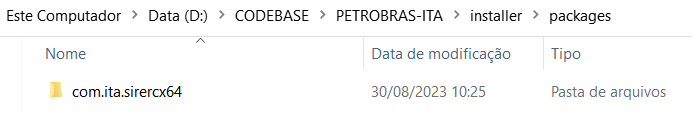
\includegraphics[width=0.75\textwidth]{images/sirercinstallerpackage.png}}
			\caption{Criação do diretório para pacote 64 bits do \sistema{}}\label{fig:sirercinstallerpackage}
		\end{figure}
		
		\item Dentro do diretório \path{com.ita.sirercx64}, crie dois subdiretórios chamados \path{data} e \path{meta} (vide Figura \ref{fig:sirercpackagedirs}). O primeiro conterá executáveis, bibliotecas e outros arquivos necessários para o funcionamento do \sistema{}. O segundo conterá informações complementares do \emph{package}.
		
		\begin{figure}[H]\centering
			\fbox{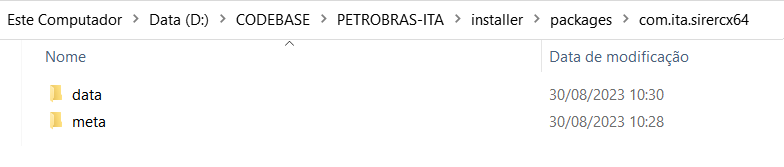
\includegraphics[width=0.75\textwidth]{images/sirercpackagedirs.png}}
			\caption{Subdiretórios \emph{data} e \emph{meta} criados}\label{fig:sirercpackagedirs}
		\end{figure}
		
		\item No diretório \path{meta}, crie um arquivo chamado \path{license.txt} contendo as informações da licença associada ao \emph{software}. A \emph{\gnu{}} (GPL) pode ser obtida em \url{https://www.gnu.org/licenses/gpl-3.0.txt}. Verifique qual licença está em uso atualmente no \sistema{}.
		
		\item Ainda no diretório \path{meta}, crie um arquivo chamado \path{package.xml} para definir os comportamentos do instalador e mensagens informativas. O conteúdo deve ser semelhante ao seguinte:
		
\begin{lstlisting}
	<?xml version="1.0" encoding="UTF-8"?>
	<Package>
	<DisplayName>SIRERC 64Bits</DisplayName>
	<Description>x64 Version</Description>
	<Version>1.0.0</Version>
	<ReleaseDate>2023-08-30</ReleaseDate>
	<Licenses>
	<License name="License Information" file="license.txt" />
	</Licenses>
	<Default>true</Default>
	</Package>
\end{lstlisting}

		
		\item Verifique as \emph{tags} aceitas neste arquivo na documentação do Qt em \url{https://doc.qt.io/qtinstallerframework/ifw-component-description.html#package-information-file-syntax}. O conteúdo apresentado é apenas um exemplo; verifique se há uma versão mais completa deste arquivo em uso no \sistema{}.
		
		\item Isso conclui a configuração dos arquivos no diretório \path{meta} (vide Figura \ref{fig:sirercpackagemeta}).
		
		\begin{figure}[H]\centering
			\fbox{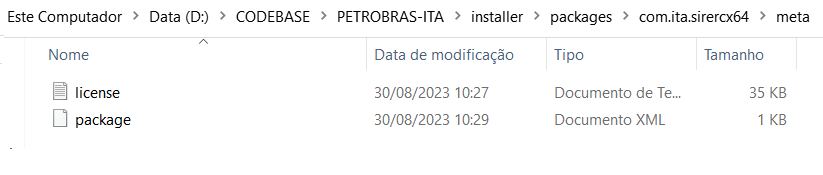
\includegraphics[width=0.75\textwidth]{images/sirercpackagemeta.png}}
			\caption{Arquivos no diretório \emph{meta}}\label{fig:sirercpackagemeta}
		\end{figure}
	\end{enumerate}
	
	\item **Preparação dos arquivos de deployment:**
	\begin{enumerate}
		\item No diretório \path{data}, crie um subdiretório chamado \path{win64} (vide Figura \ref{fig:sirercdatawin64}). Copie para este diretório o arquivo \emph{.exe} gerado pelo \qtcreator{} ou outra IDE usada para desenvolver o \sistema{} (vide Figura \ref{fig:sirercdataexe}). Este arquivo normalmente está localizado nos diretórios de \path{build} criados durante o desenvolvimento.
		
		\begin{figure}[H]\centering
			\fbox{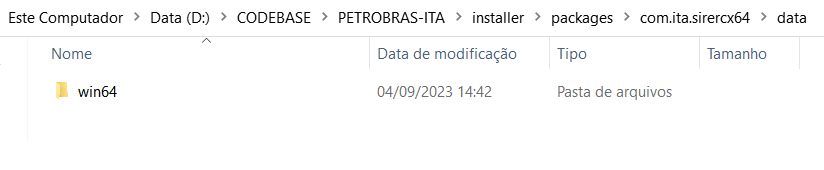
\includegraphics[width=0.75\textwidth]{images/sirercdatawin64.png}}
			\caption{Criação do subdiretório \emph{win64} dentro de \emph{data}}\label{fig:sirercdatawin64}
		\end{figure}
		
		\begin{figure}[H]\centering
			\fbox{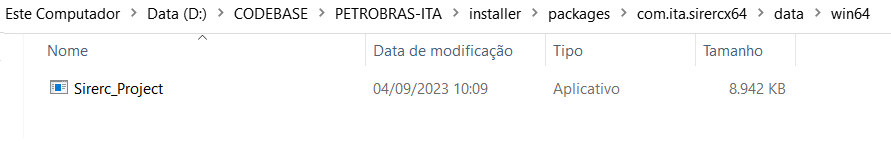
\includegraphics[width=0.75\textwidth]{images/sirercdataexe.png}}
			\caption{Arquivo \emph{.exe} no diretório \emph{win64}}\label{fig:sirercdataexe}
		\end{figure}
		
		\item O diretório \path{win64} deve conter todos os executáveis, bibliotecas e dependências necessárias para executar o \sistema{}. O Qt possui uma ferramenta de \emph{deploy} que traz todas essas dependências para o diretório a partir do arquivo executável \emph{.exe}. Para acessar essa ferramenta, abra um terminal no \emph{Powershell} do \emph{\windows{}} e navegue até o diretório \path{win64}.
		
		\item No terminal \emph{Powershell}, certifique-se de estar no diretório que contém o executável do \sistema{} copiado anteriormente. Execute o comando a seguir, substituindo a variável \path{${QtDirectory}} pelo caminho onde o Qt está instalado e usando o nome correto do arquivo \emph{.exe}:
		
		\begin{verbatim}
			${QtDirectory}\5.15.2\msvc2015_64\bin\windeployqt.exe Sirerc_Project.exe --compiler-runtime
		\end{verbatim}
		
		\item Aguarde a conclusão do processo de \emph{deploy} e verifique se há uma grande quantidade de novos arquivos e diretórios dentro do diretório \path{win64} (vide Figura \ref{fig:sirercdeploy}).
		
		\begin{figure}[H]\centering
			\fbox{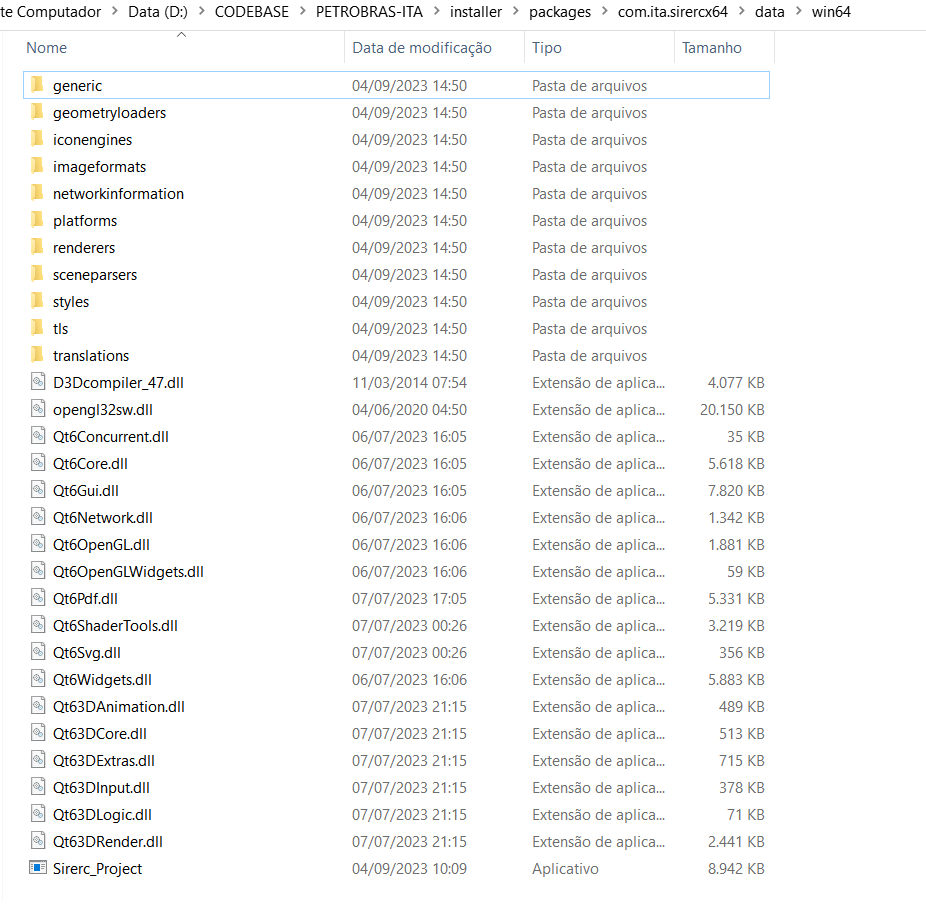
\includegraphics[width=0.75\textwidth]{images/sirercdeploy.png}}
			\caption{Diretório \emph{win64} após o \emph{deploy}}\label{fig:sirercdeploy}
		\end{figure}
	\end{enumerate}
	
	\item **Resolução de dependências extras:**
	\begin{enumerate}
		\item Na data de escrita deste documento, a ferramenta de \emph{deploy} não consegue encontrar algumas dependências extras do \sistema{}, como as bibliotecas do VTK. Essas e outras dependências devem ser rastreadas usando ferramentas como a disponível em \url{https://github.com/lucasg/Dependencies}.
		\item A ferramenta \emph{Dependencies} possui uma interface de usuário que permite fornecer um arquivo executável \emph{.exe} e receber uma lista de todas as dependências (\emph{.dlls}) necessárias para o funcionamento deste executável (vide Figura \ref{fig:deptool}).
		
		\begin{figure}[H]\centering
			\fbox{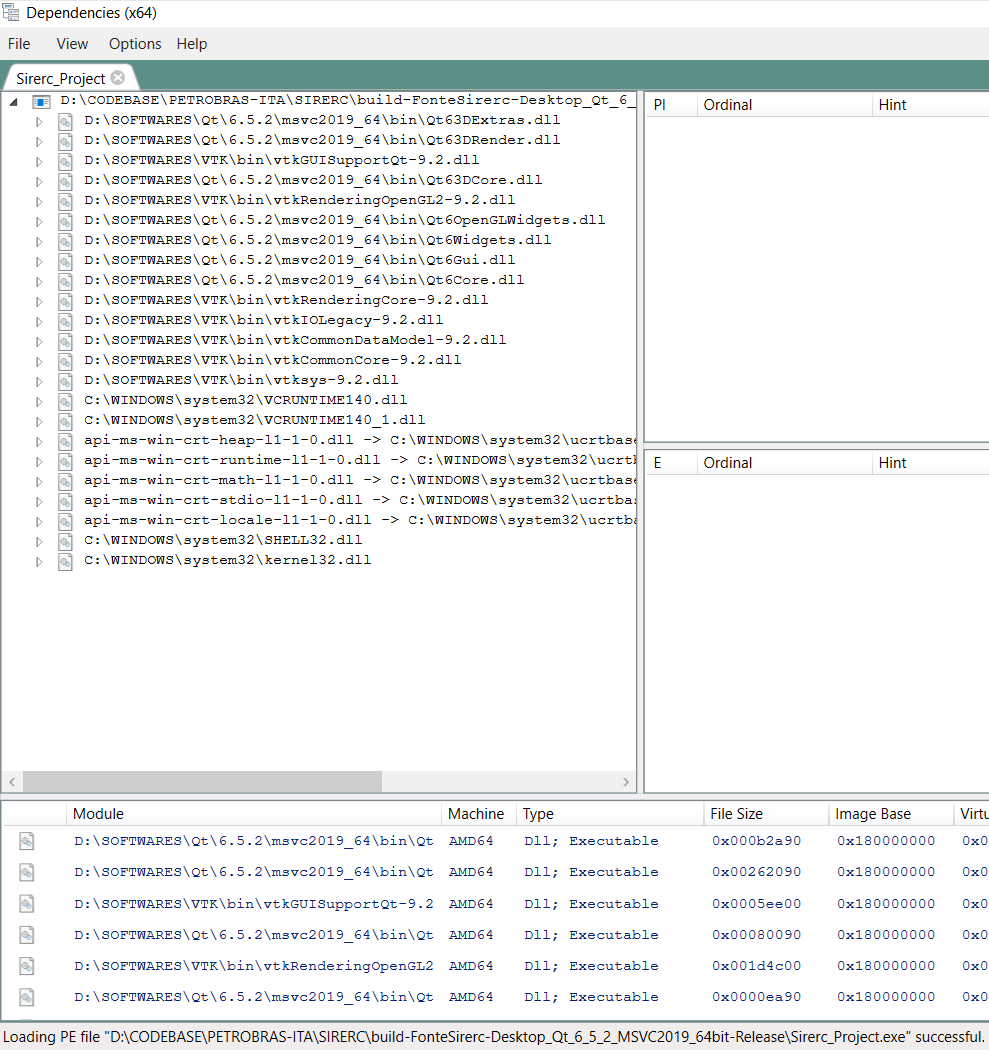
\includegraphics[width=0.75\textwidth]{images/deptool.png}}
			\caption{Dependências do \sistema{} encontradas com a ferramenta \emph{Dependencies}}\label{fig:deptool}
		\end{figure}
		
		\item Copie todas as dependências necessárias para o diretório \path{win64}, incluindo bibliotecas do VTK, por exemplo.
		
		\cautionbox{Este processo deve ser realizado com cautela, pois sem todas as dependências necessárias, o \sistema{} não funcionará corretamente após a instalação.}
	\end{enumerate}
	
	\item **Geração do instalador:**
	\begin{enumerate}
		\item Após a resolução de todas as dependências, você pode gerar o instalador. Para isso, abra novamente um terminal \emph{Powershell} e acesse o diretório principal do instalador, onde estão os diretórios \path{config} e \path{packages}.
		\item Nesse diretório, execute o seguinte comando para gerar o instalador, substituindo a variável \path{${QtDirectory}} pelo caminho onde o Qt está instalado:
		
		\begin{verbatim}
			${QtDirectory}\Tools\QtInstallerFramework\4.6\bin\binarycreator.exe -c config\config.xml -p packages\ -f SirercInstaller
		\end{verbatim}
		
		\item Aguarde a geração do instalador. Se o processo for bem-sucedido, o terminal \emph{Powershell} não exibirá nenhuma saída, mas você encontrará um novo executável \emph{SirercInstaller.exe} no diretório do instalador (vide Figura \ref{fig:sirercinstallerfinish}). Este é o arquivo que deve ser fornecido para instalação nas máquinas dos usuários (vide Figura \ref{fig:sirercinstaller}).
		
		\begin{figure}[H]\centering
			\fbox{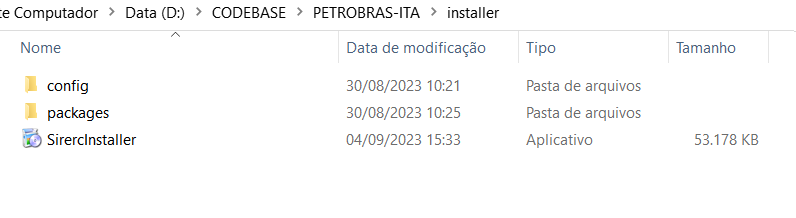
\includegraphics[width=0.75\textwidth]{images/sirercinstallerfinish.png}}
			\caption{Instalador gerado para o \sistema{}}\label{fig:sirercinstallerfinish}
		\end{figure}
		
		\begin{figure}[H]\centering
			\fbox{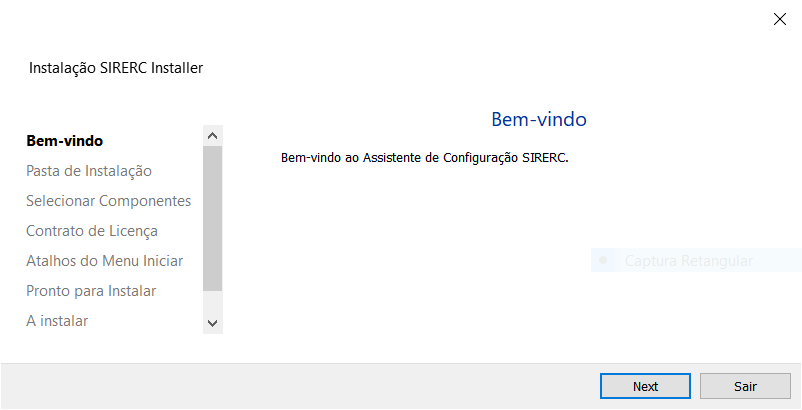
\includegraphics[width=0.75\textwidth]{images/sirercinstaller.png}}
			\caption{Execução do instalador do \sistema{}}\label{fig:sirercinstaller}
		\end{figure}
	\end{enumerate}
\end{enumerate}



\end{document}